\section{Evaluation}

\begin{frame}{Evaluation}
    \begin{itemize}
        \item Accelerometer-based gesture detection inspired by \textit{uWave} \cite{liu2009uwave}

        \item 14 records of three-dimensional acceleration time series by 14 different experimentees

        \item Recorded via a Wii Remote\texttrademark~Plus controller
        \begin{center}
            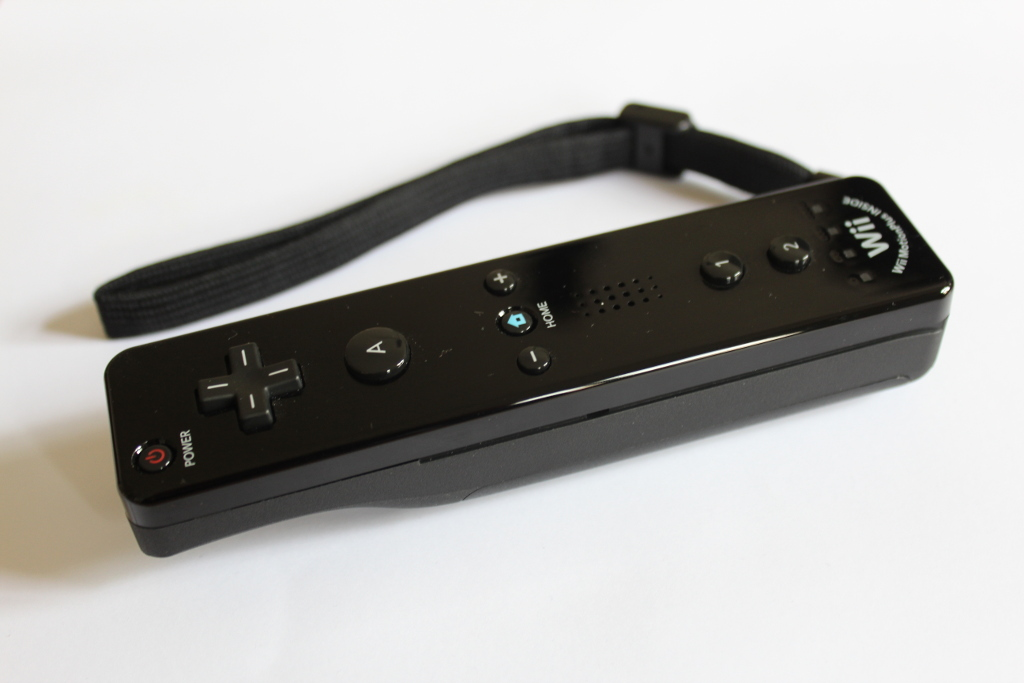
\includegraphics[width=0.5\textwidth]{wii-remote-plus-controller.JPG}
        \end{center}
    \end{itemize}
\end{frame}

\begin{frame}{Evaluation}{Data Recording Instructions}
    \begin{center}
        \resizebox {\textwidth} {!} {
            \begin{tabular}{ccccc}
                \frame{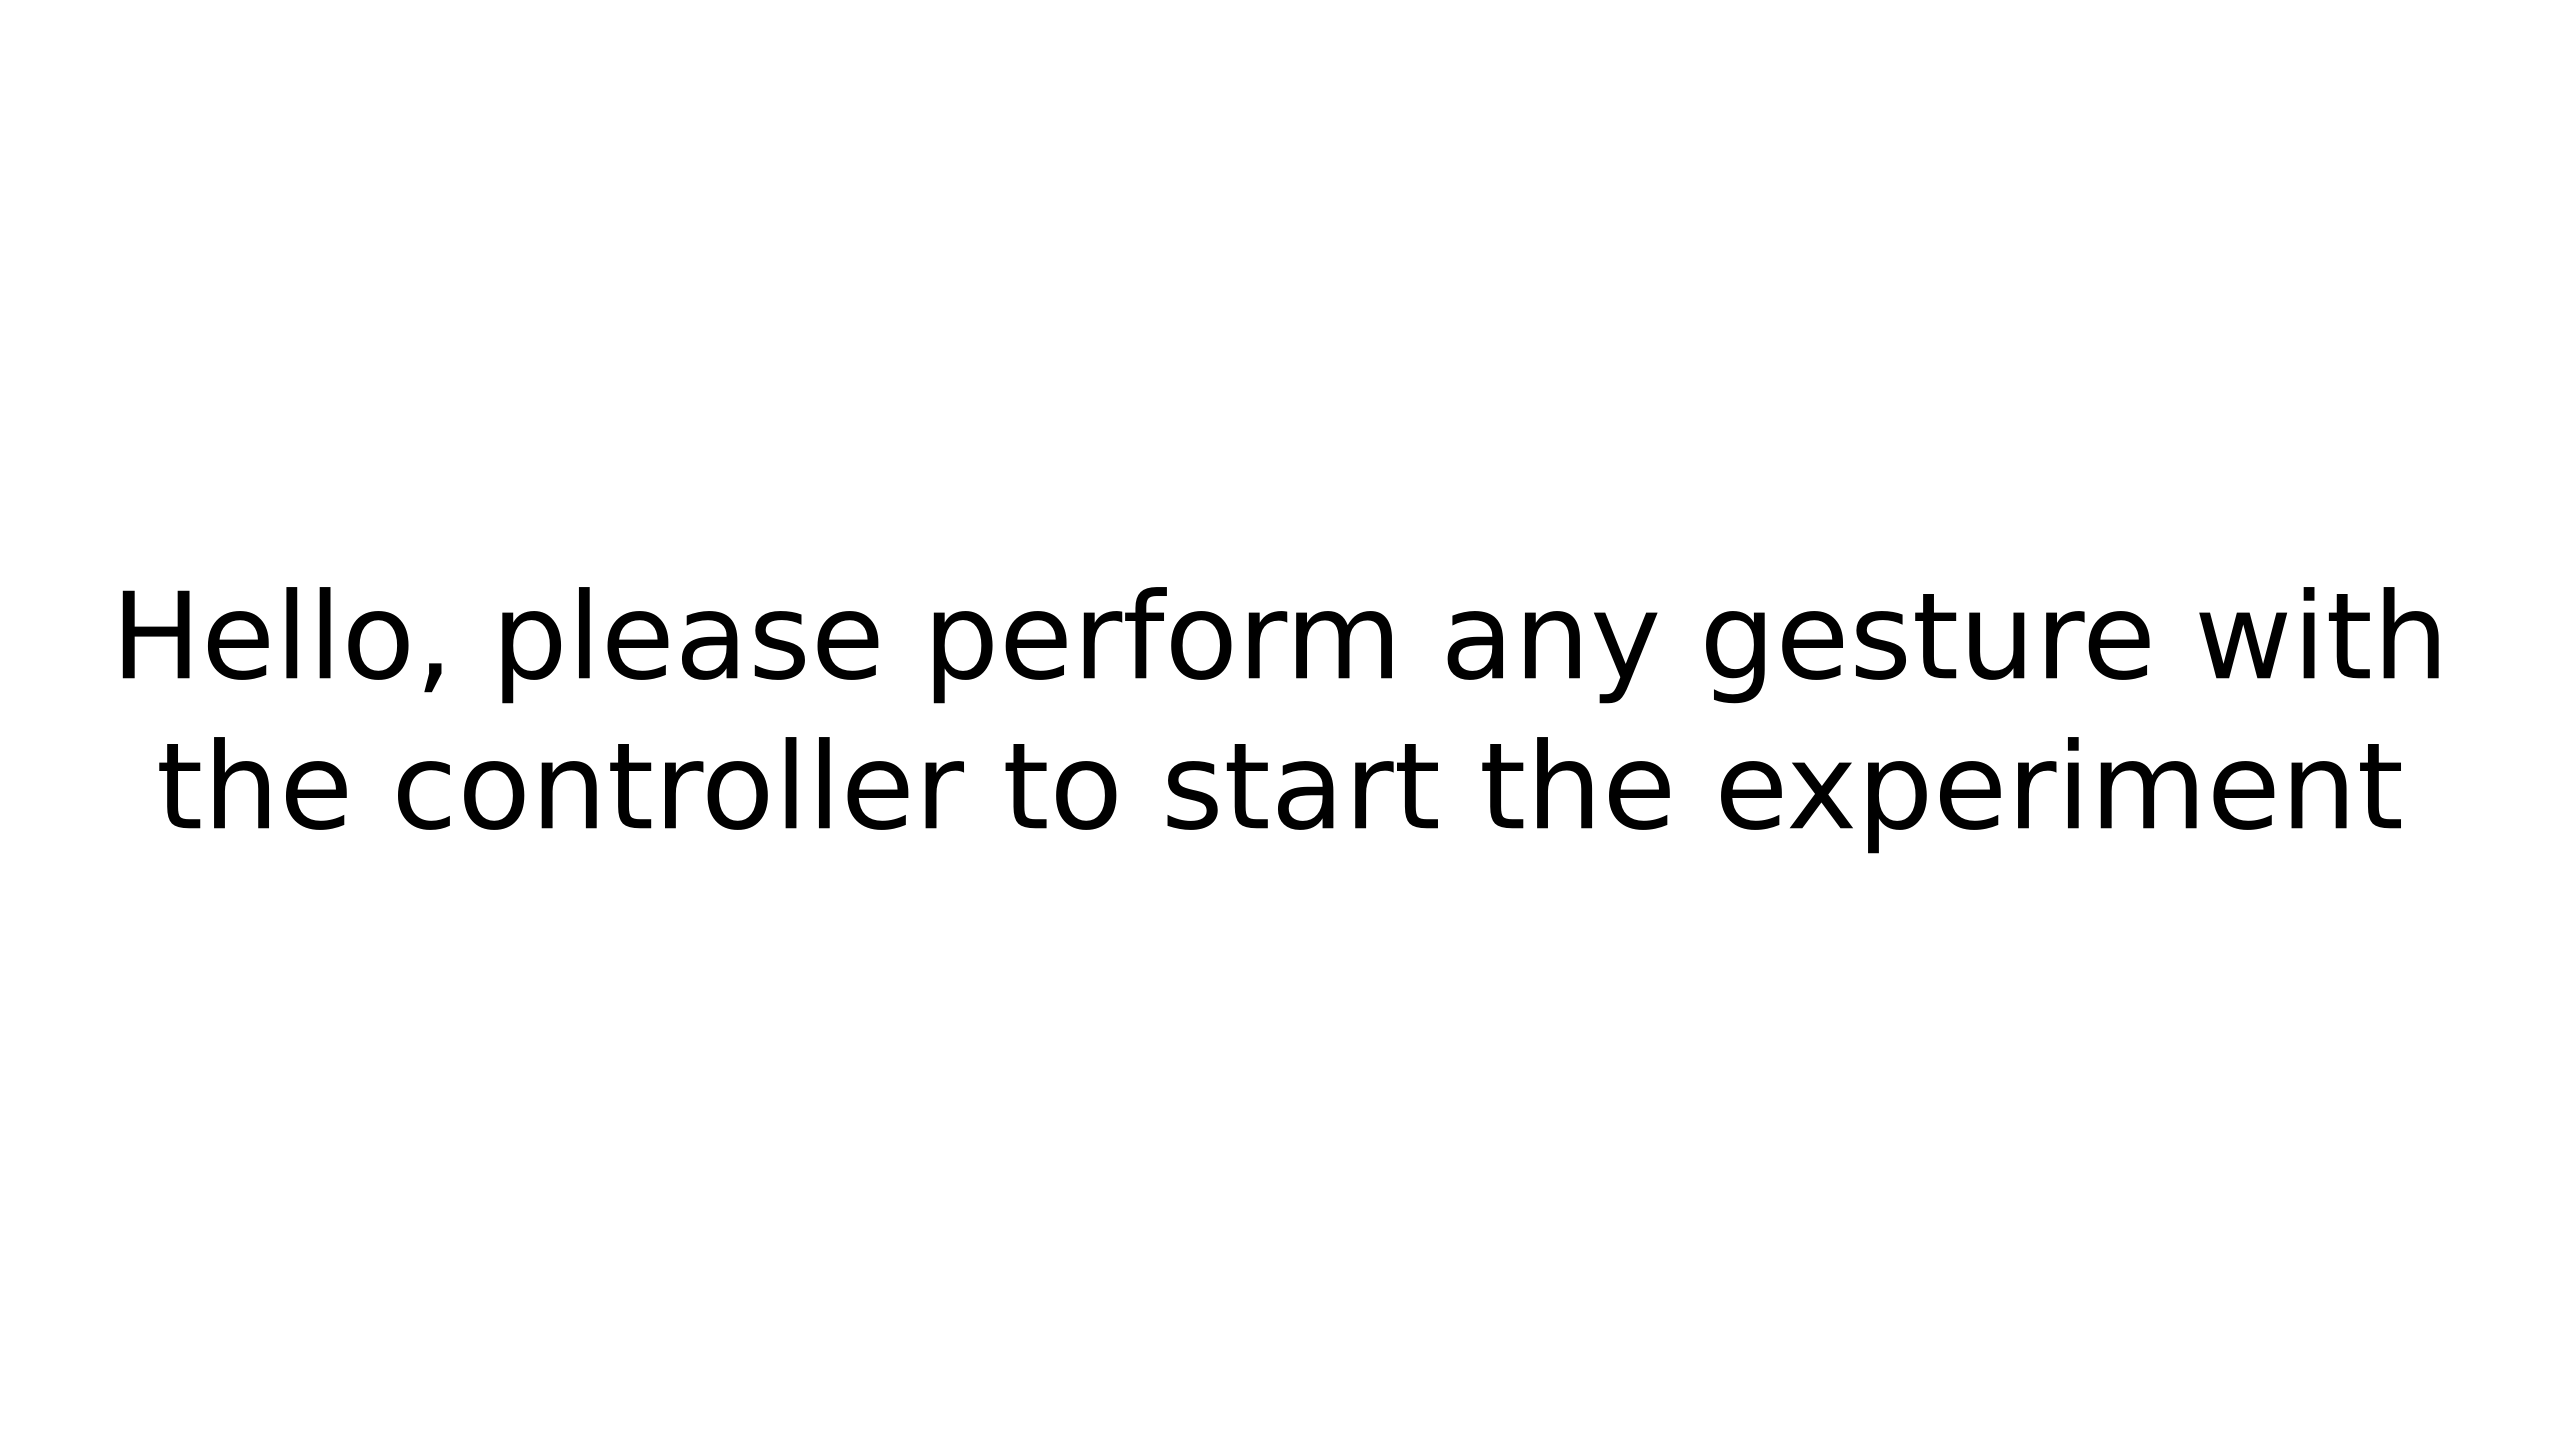
\includegraphics[width=0.25\textwidth]{1.png}} &
                \frame{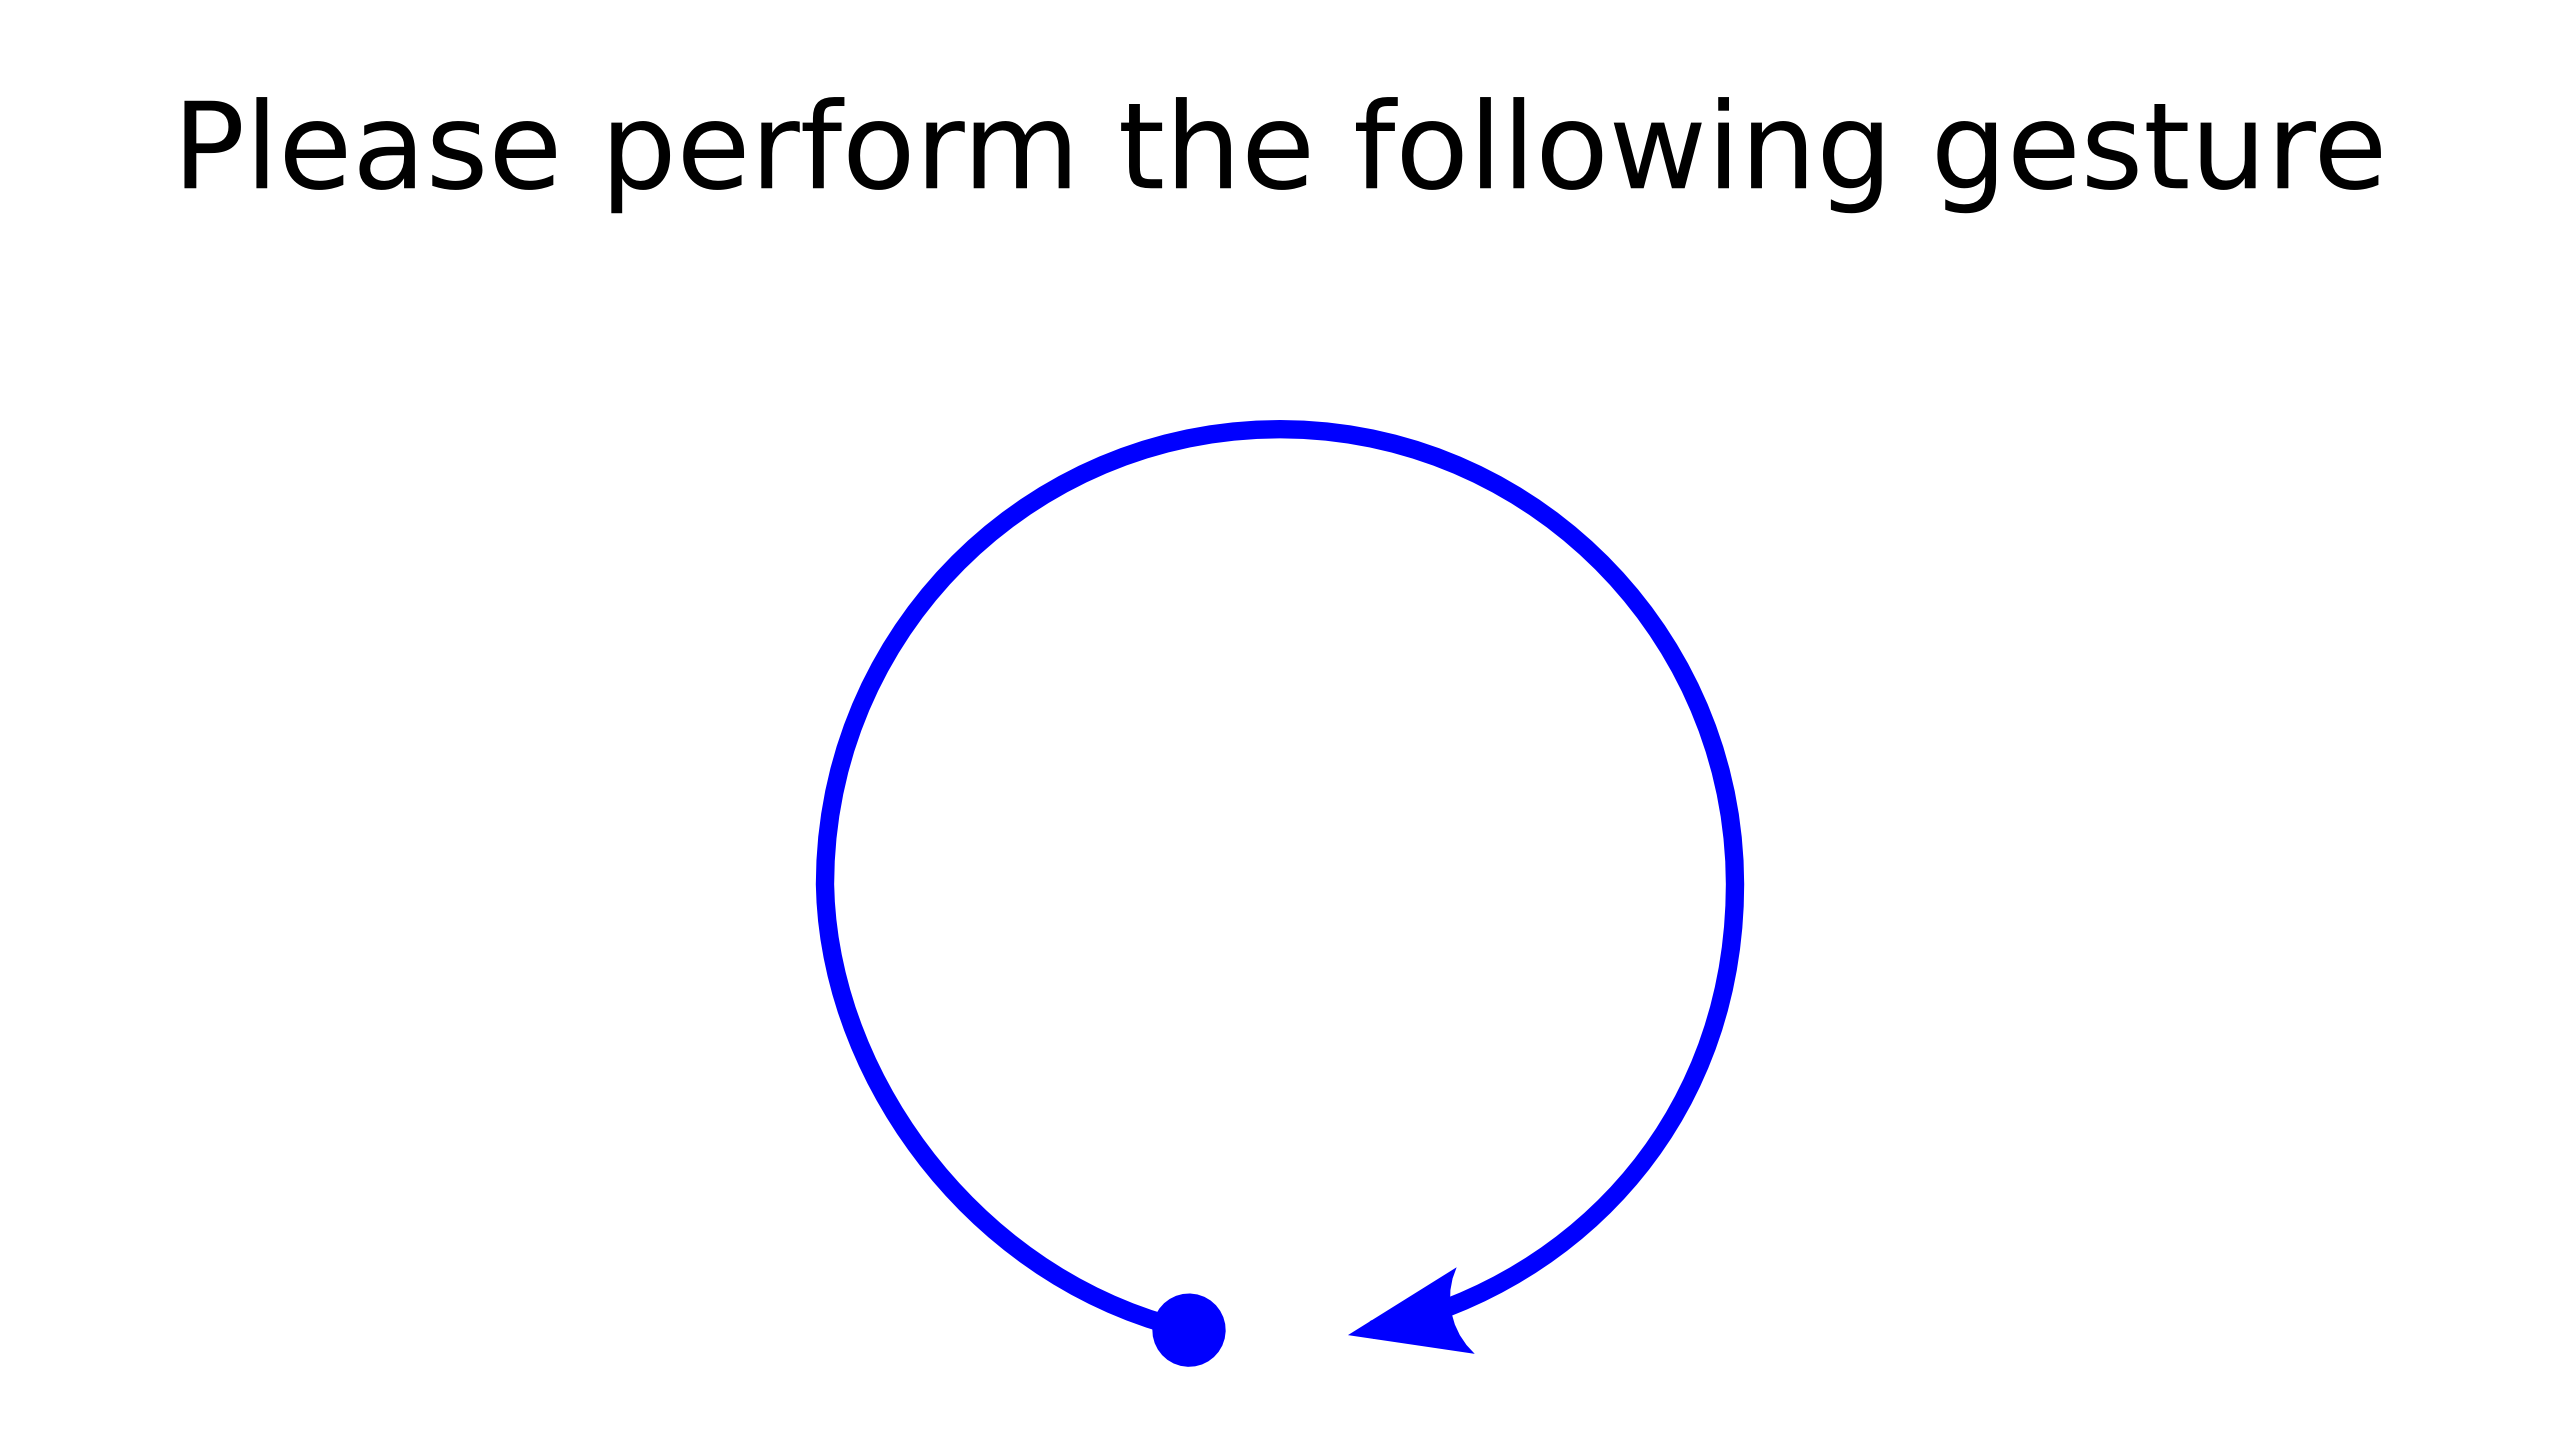
\includegraphics[width=0.25\textwidth]{2.png}} &
                \frame{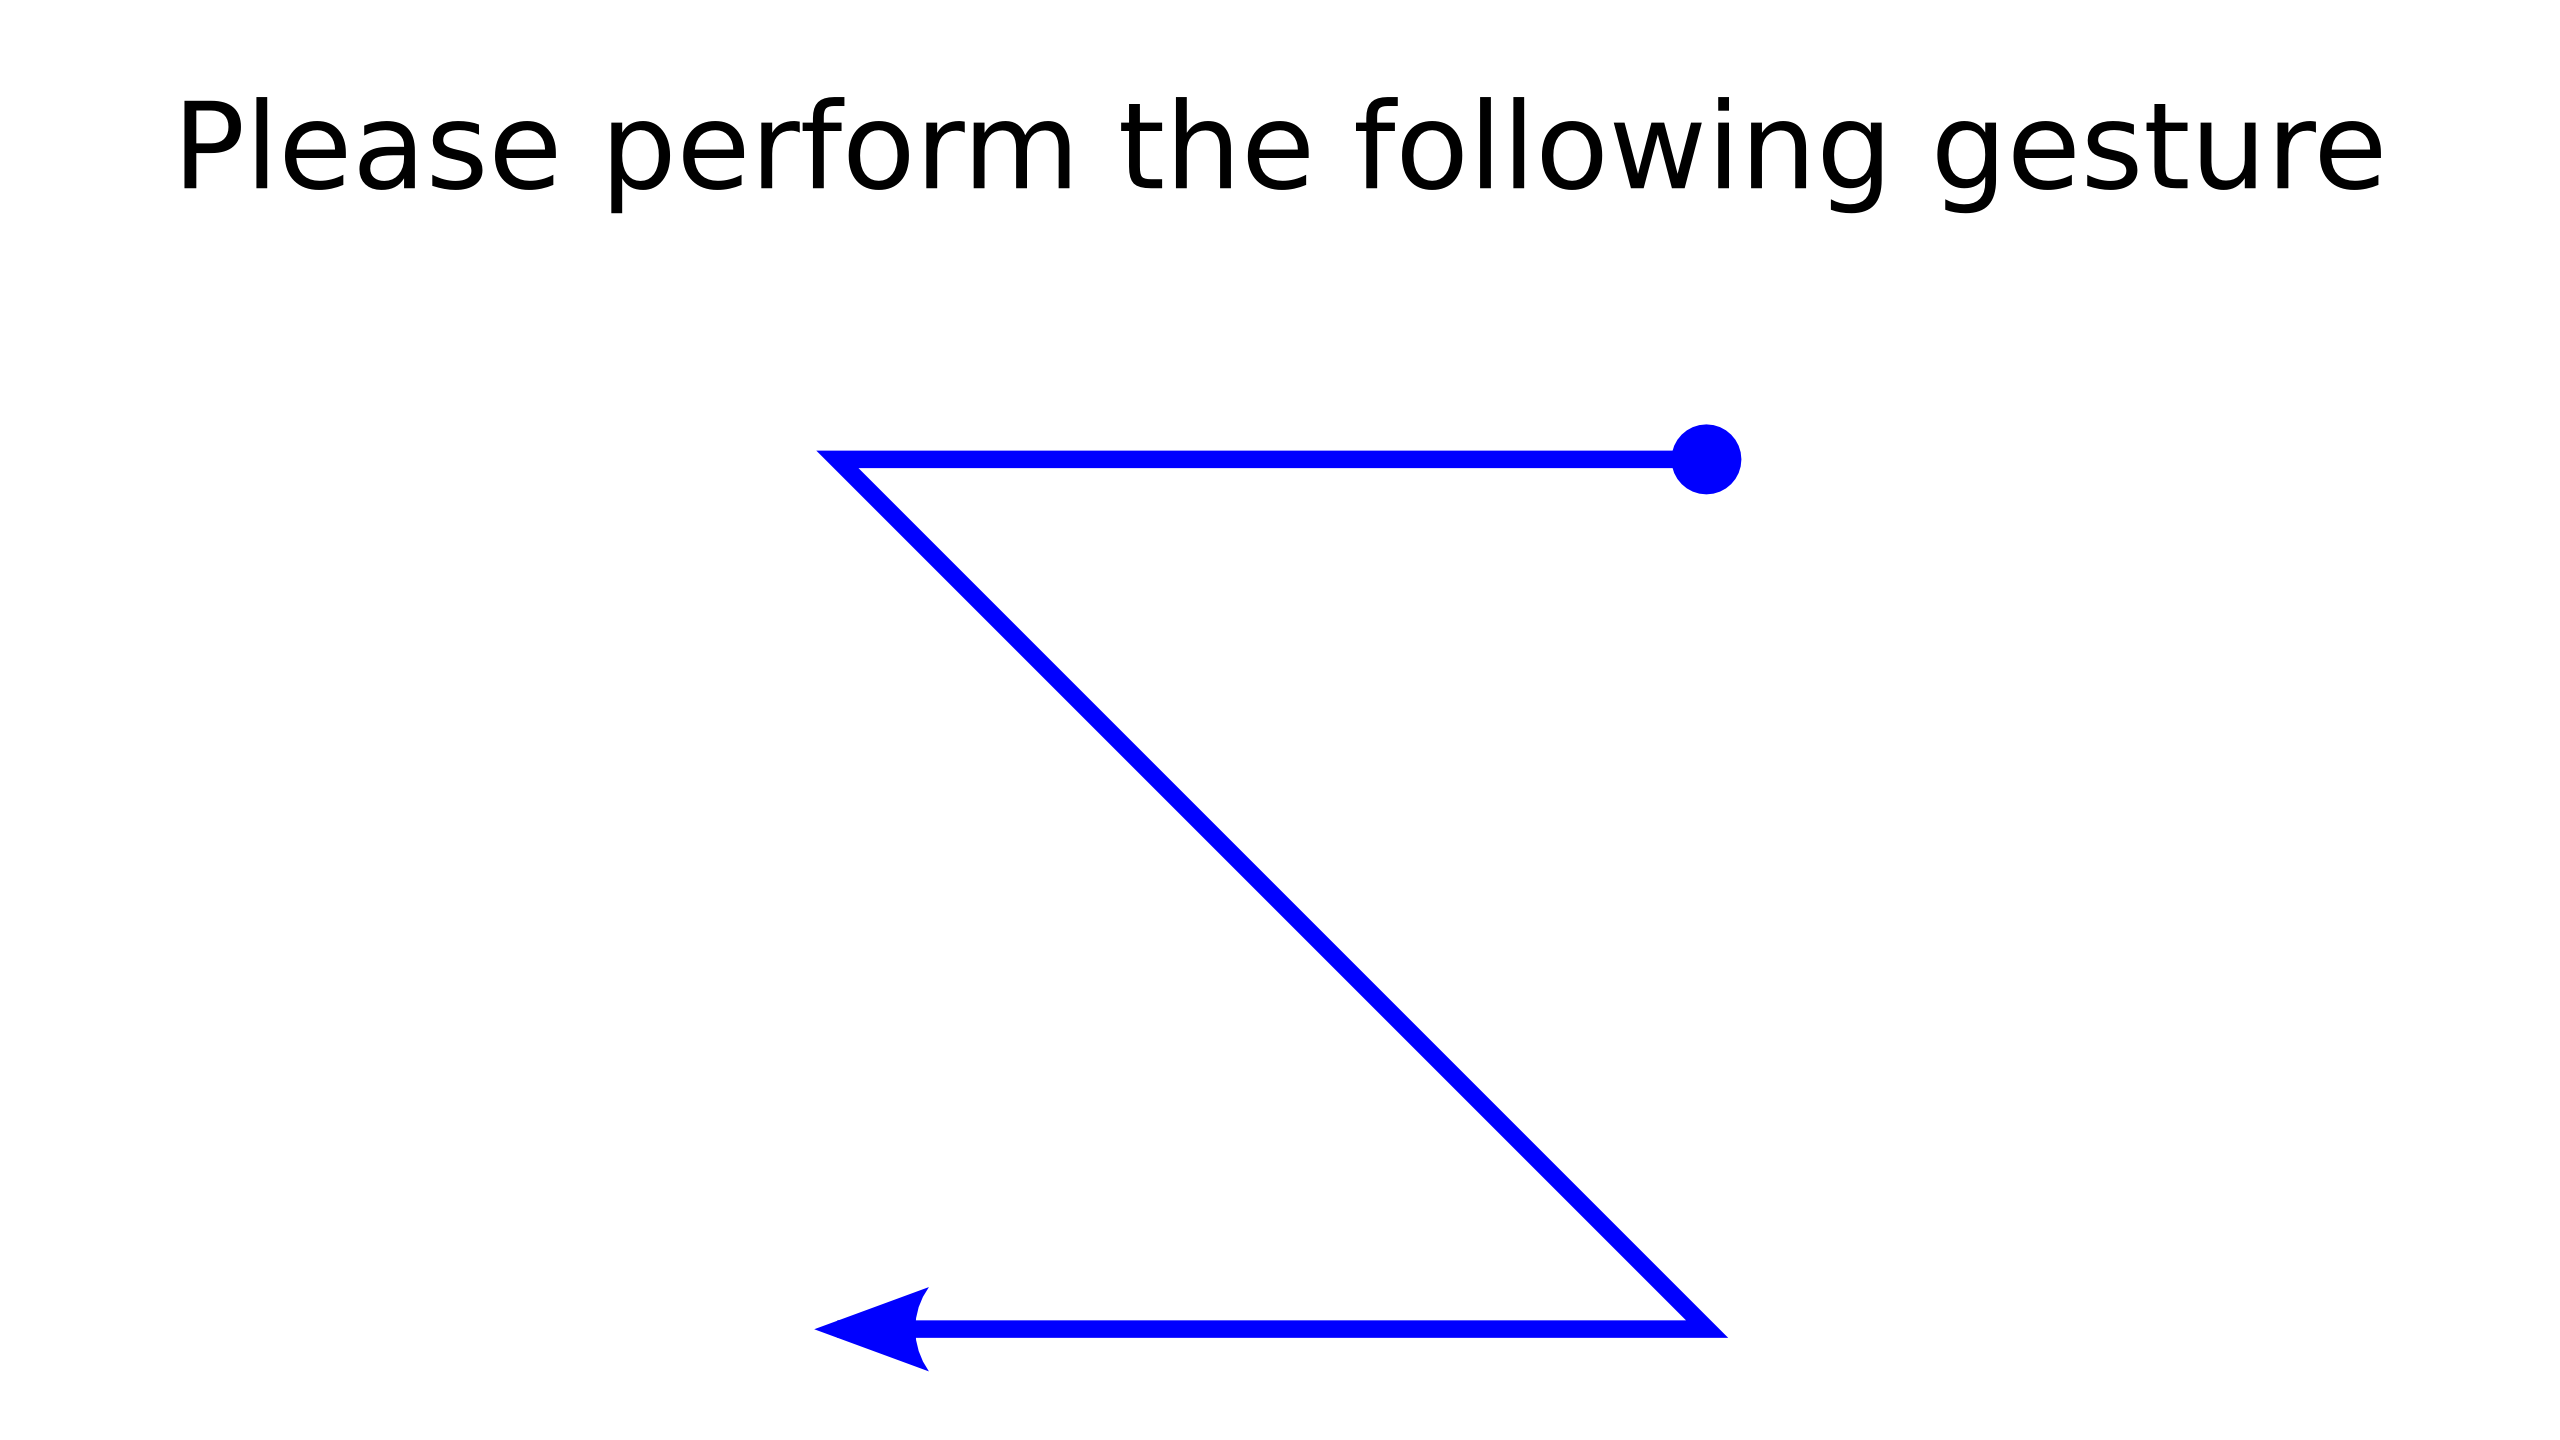
\includegraphics[width=0.25\textwidth]{3.png}} &
                \frame{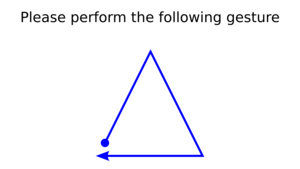
\includegraphics[width=0.25\textwidth]{4.png}} &
                \frame{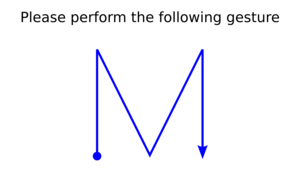
\includegraphics[width=0.25\textwidth]{5.png}} \\
                \frame{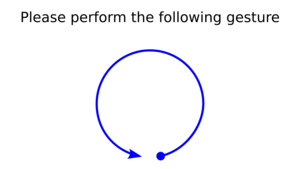
\includegraphics[width=0.25\textwidth]{6.png}} &
                \frame{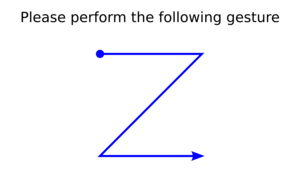
\includegraphics[width=0.25\textwidth]{7.png}} &
                \frame{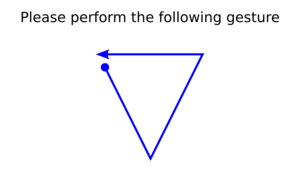
\includegraphics[width=0.25\textwidth]{8.png}} &
                \frame{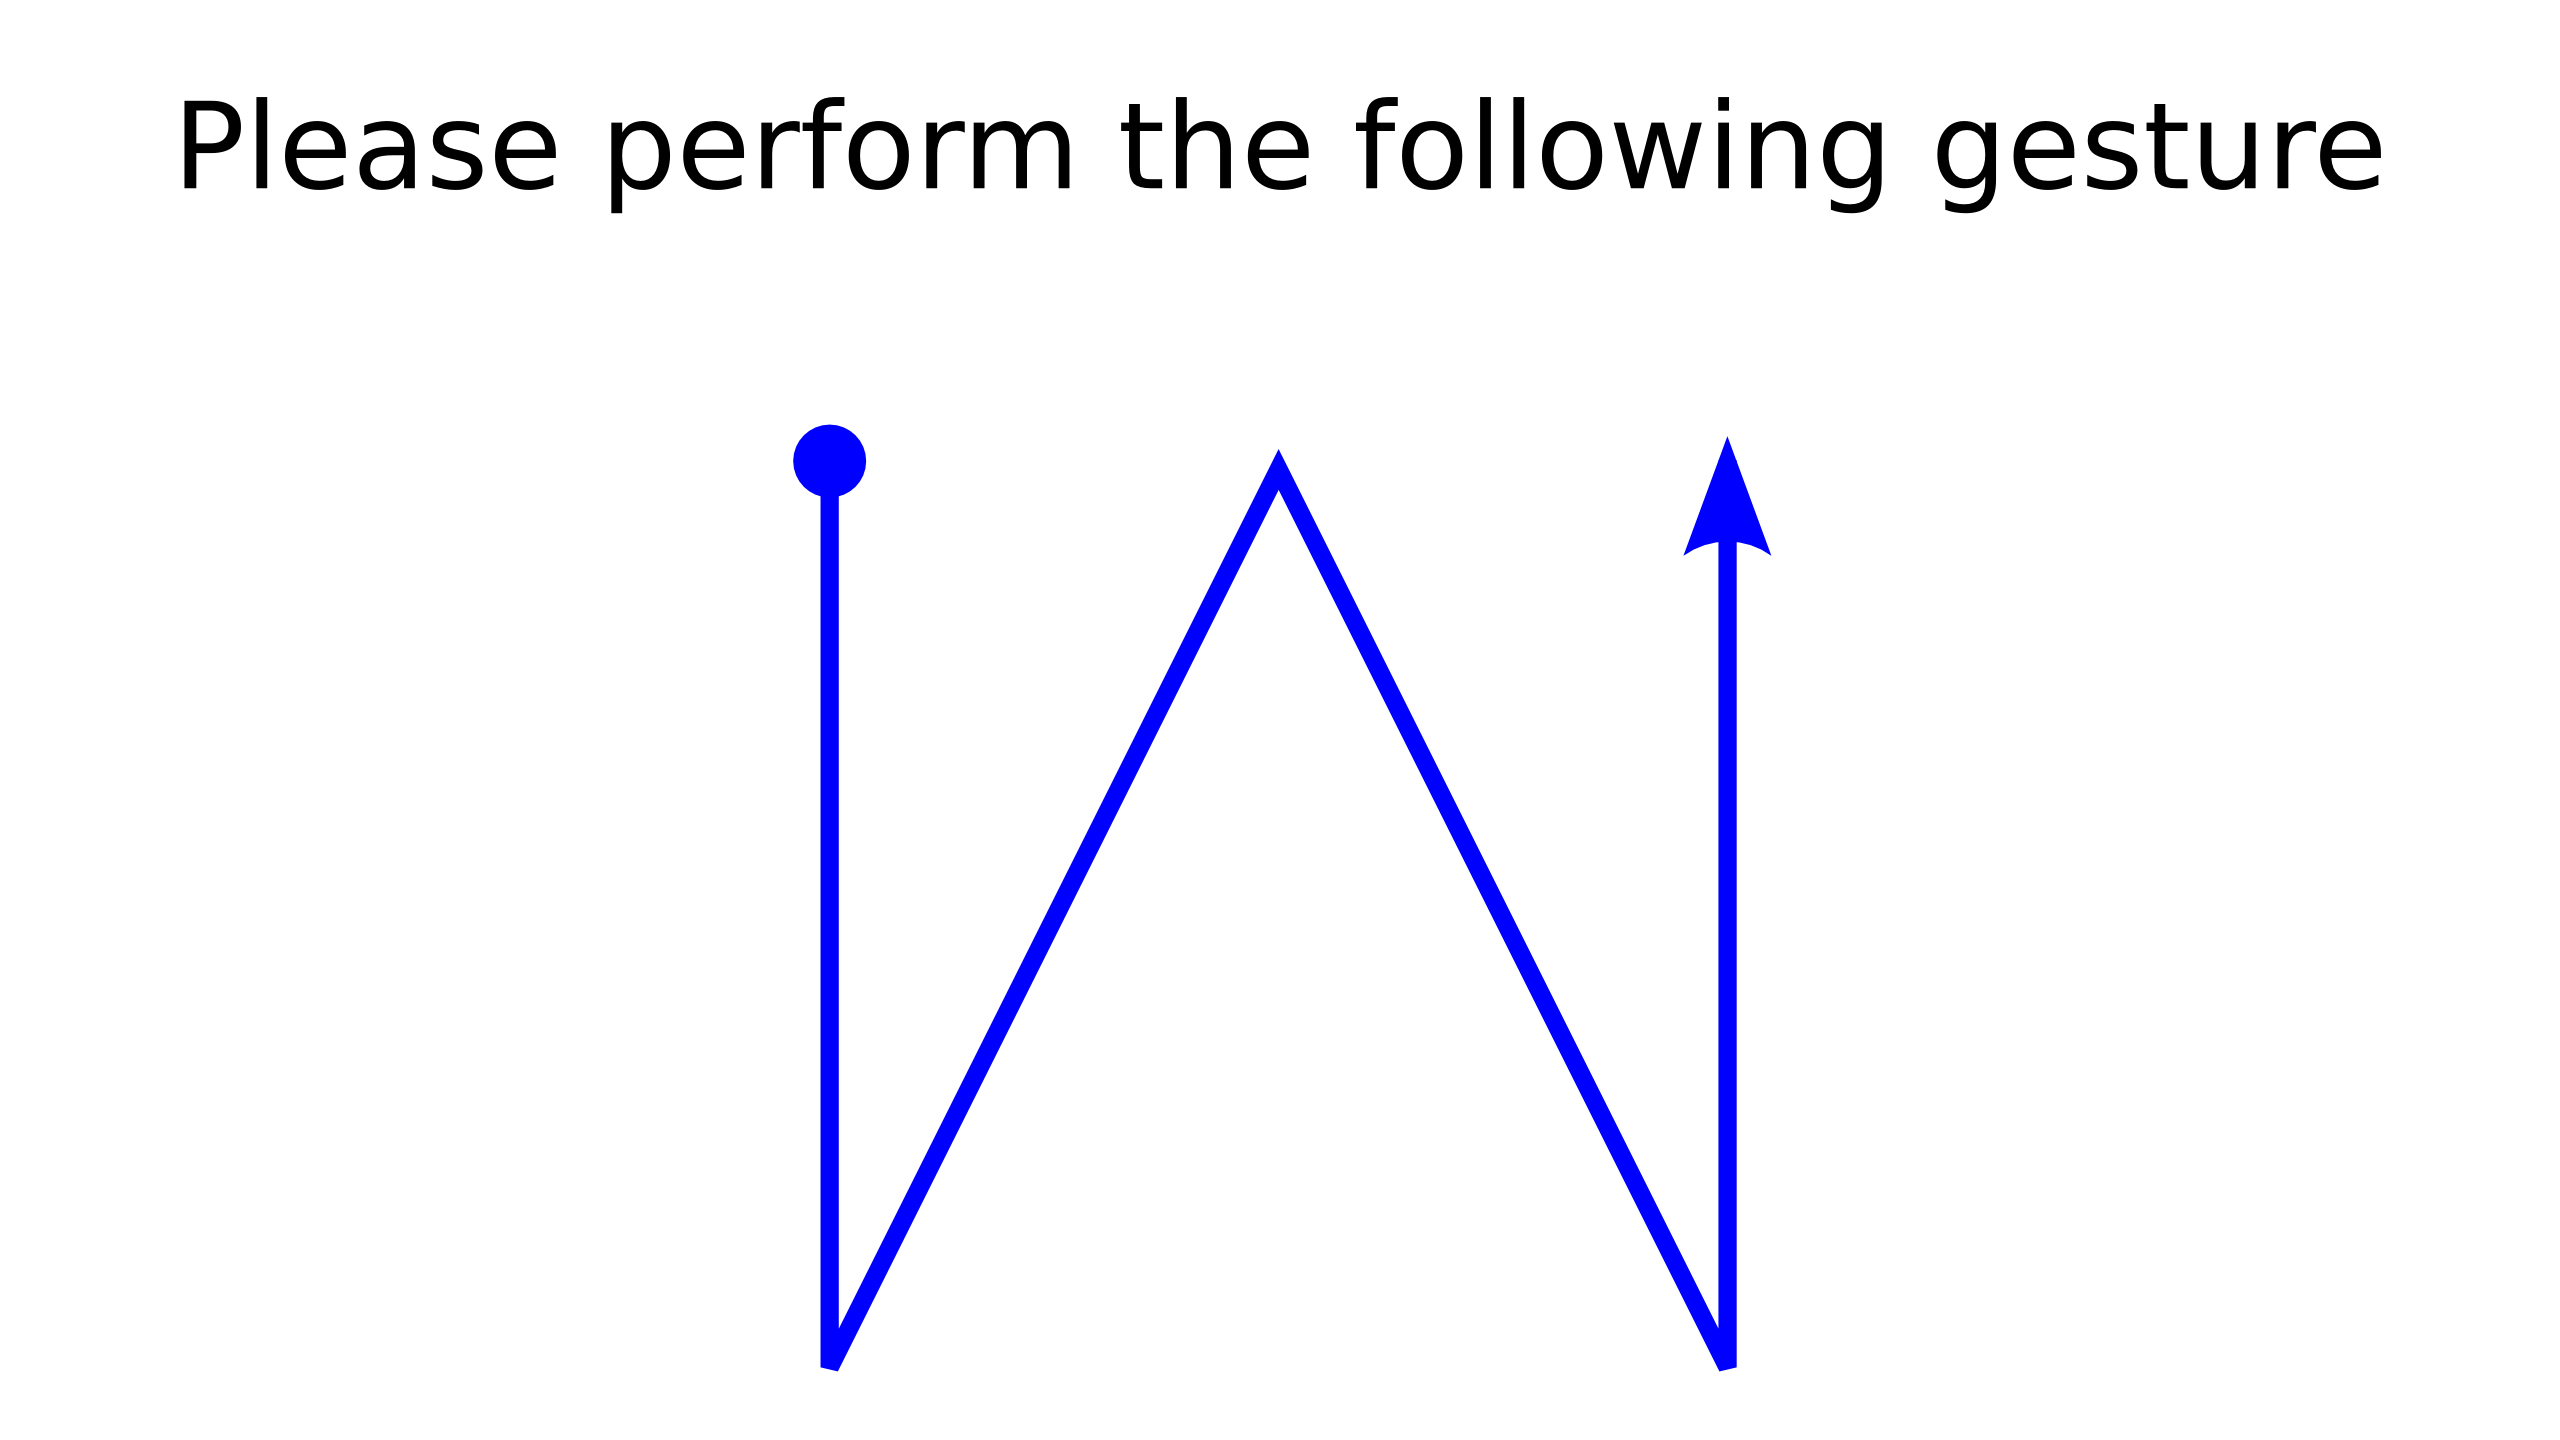
\includegraphics[width=0.25\textwidth]{9.png}} &
                \frame{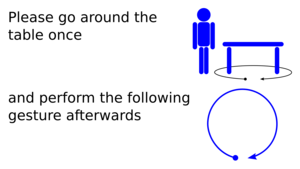
\includegraphics[width=0.25\textwidth]{10.png}} \\
                \frame{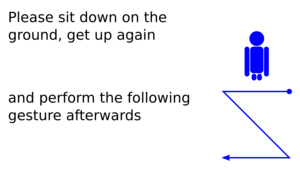
\includegraphics[width=0.25\textwidth]{11.png}} &
                \frame{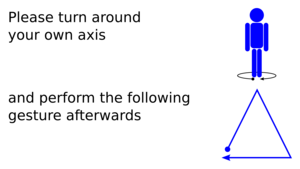
\includegraphics[width=0.25\textwidth]{12.png}} &
                \frame{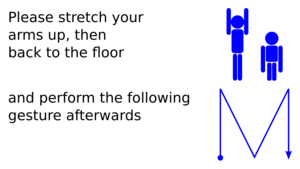
\includegraphics[width=0.25\textwidth]{13.png}} &
                \frame{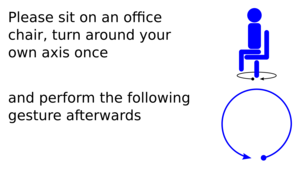
\includegraphics[width=0.25\textwidth]{14.png}} &
                \frame{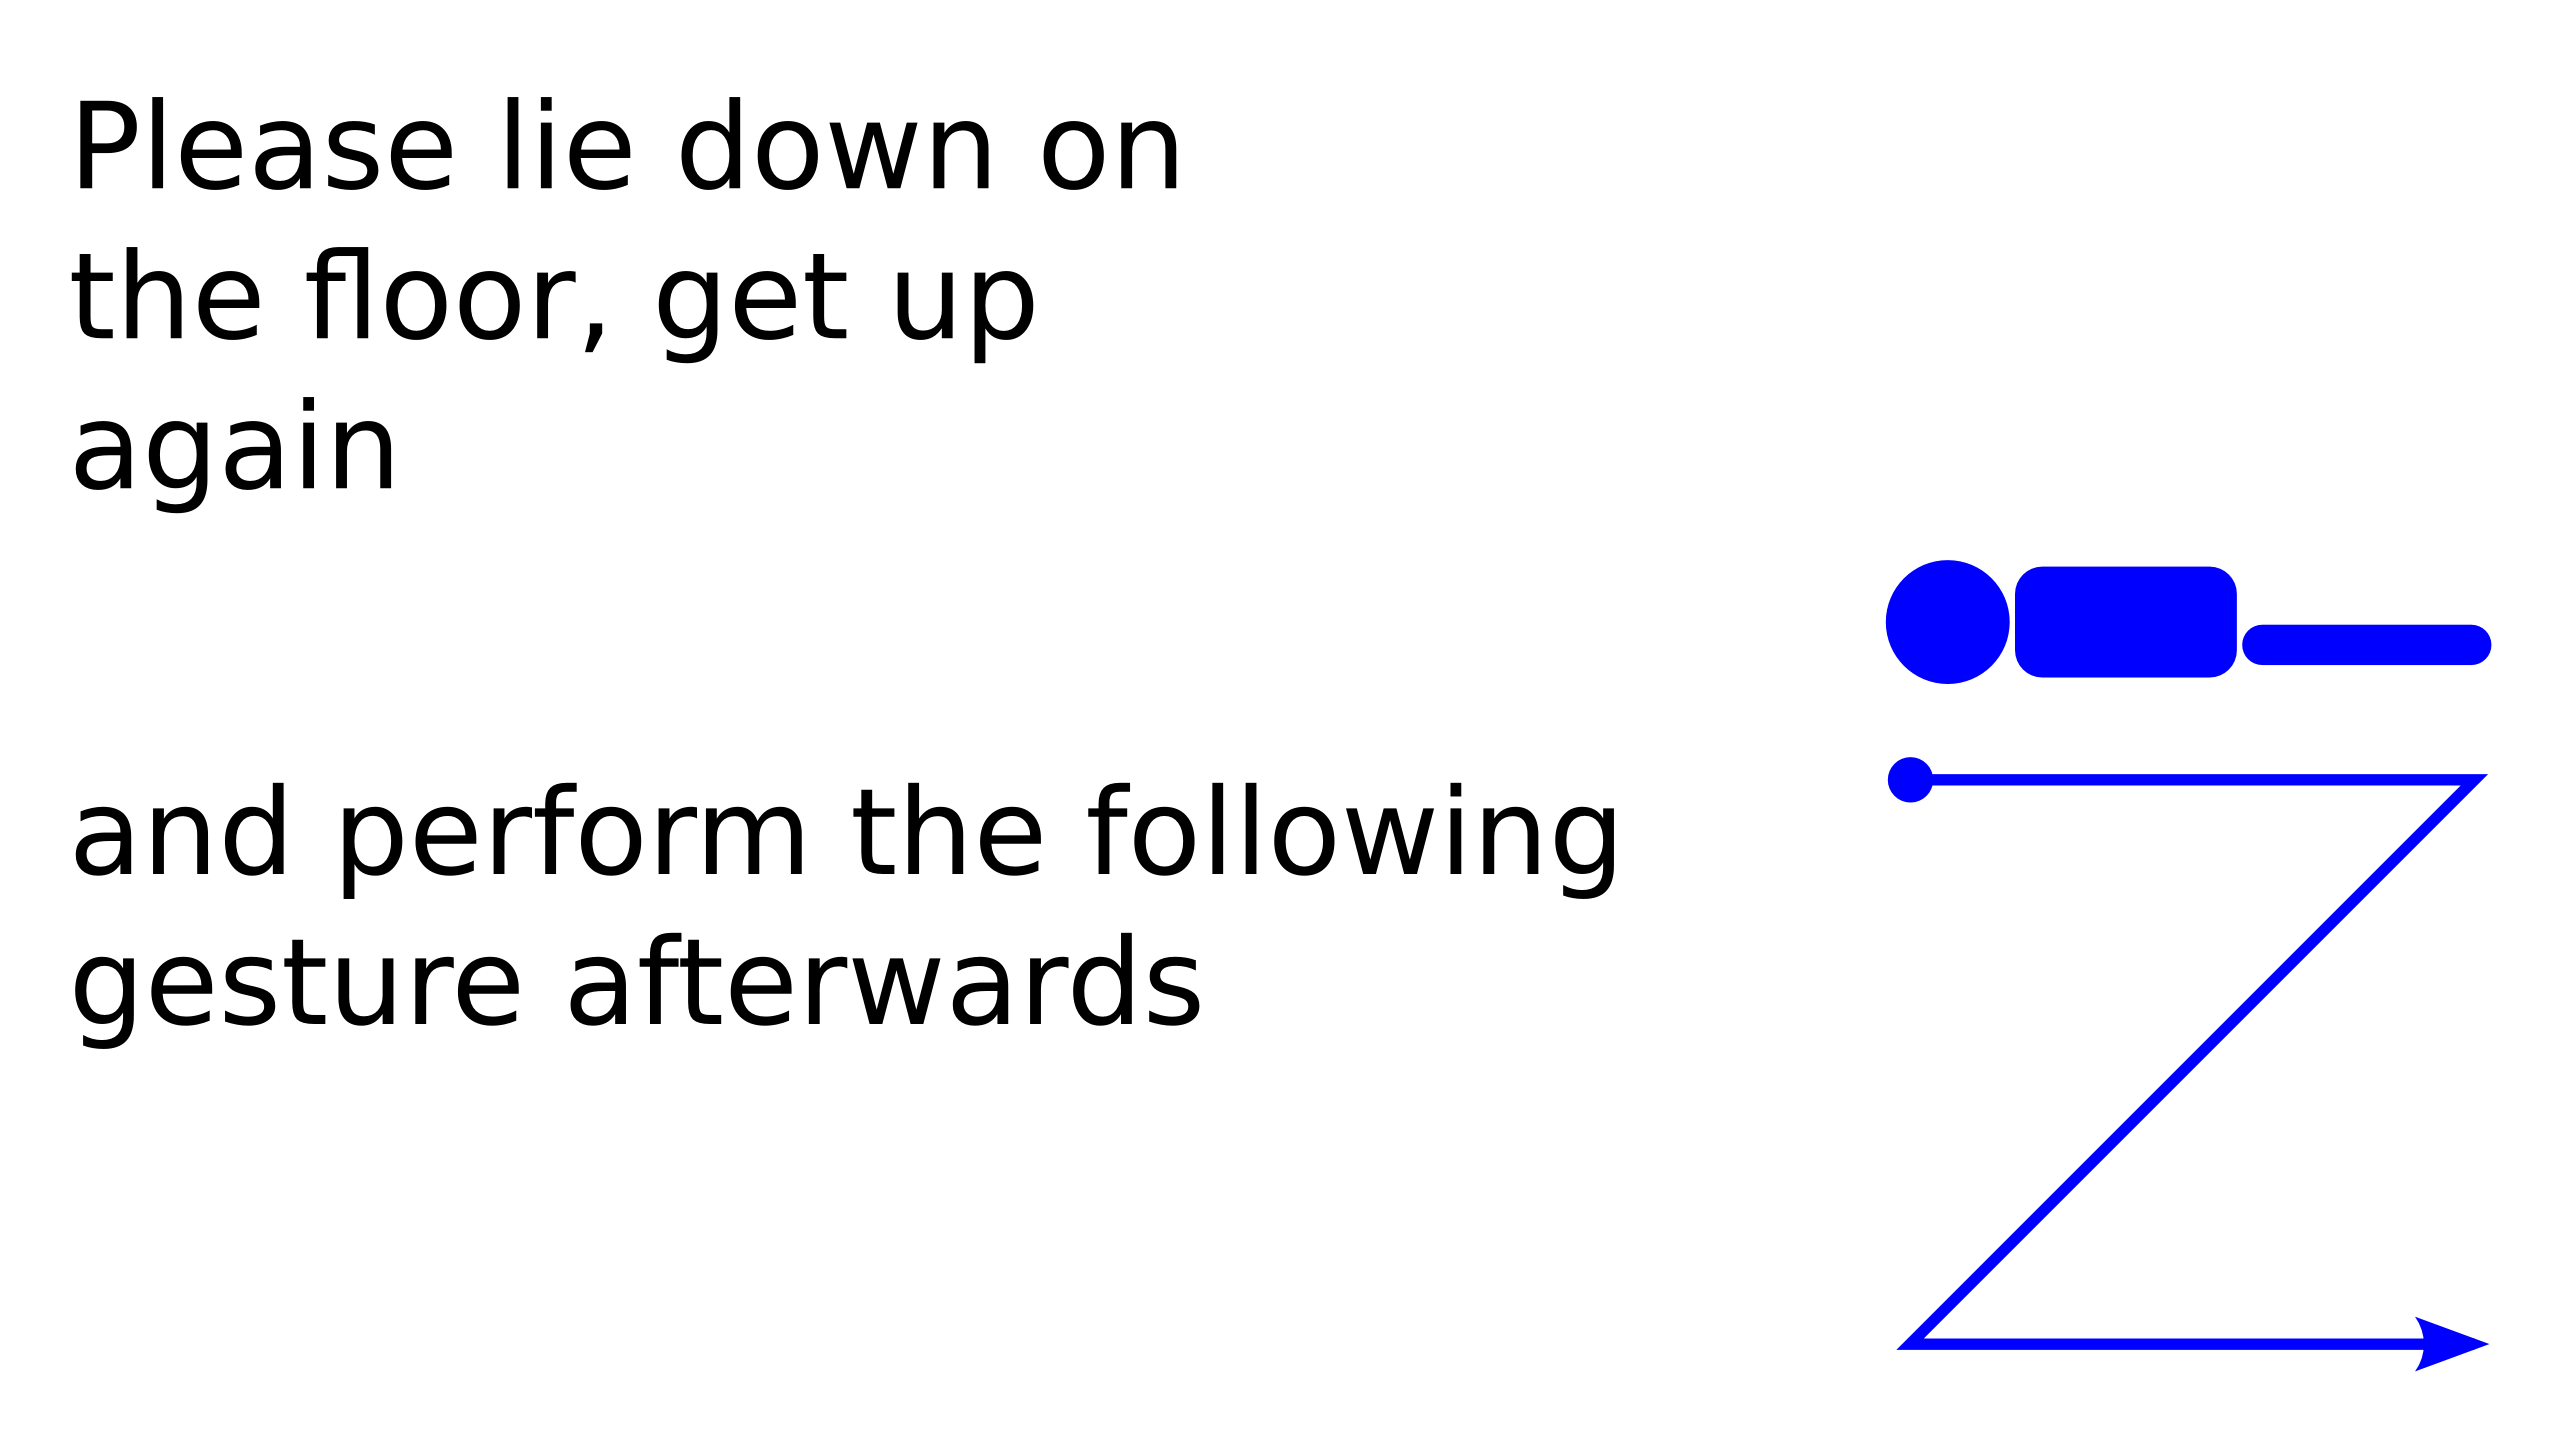
\includegraphics[width=0.25\textwidth]{15.png}} \\
                \frame{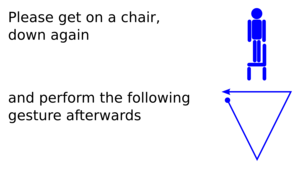
\includegraphics[width=0.25\textwidth]{16.png}} &
                \frame{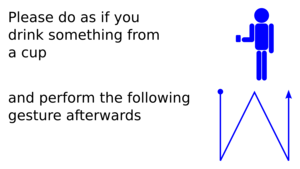
\includegraphics[width=0.25\textwidth]{17.png}} &
                \frame{
\includegraphics[width=0.25\textwidth]{18.png}} &
                \frame{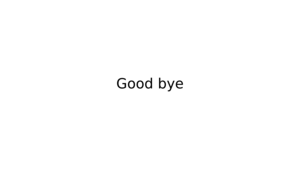
\includegraphics[width=0.25\textwidth]{19.png}} \\
            \end{tabular}
        }
    \end{center}
\end{frame}

\begin{frame}{Evaluation}{Recording Example}
    \resizebox {\textwidth} {!} {
        \begin{tikzpicture}
            \begin{axis}[
                xmin=0,
                xmax=3176,
                ymin=-16,
                ymax=16,
                width=10*\axisdefaultwidth,
                height=\axisdefaultheight,
                xticklabels={,,},
                yticklabels={,,}]
                \addplot[blue, mark=none, opacity=0.4] table[x=t, y=x] {../data/fig/record1/timeseries.dat};
                \addplot[red, mark=none, opacity=0.4] table[x=t, y=y] {../data/fig/record1/timeseries.dat};
                \addplot[green, mark=none, opacity=0.4] table[x=t, y=z] {../data/fig/record1/timeseries.dat};
                \addplot+[fill, opacity=0.5, blue, mark=none] coordinates {(38, -16) (89, -16) (89, 16) (38, 16)} --cycle;
                \addplot+[fill, opacity=0.5, blue, mark=none] coordinates {(123, -16) (177, -16) (177, 16) (123, 16)} --cycle;
                \addplot+[fill, opacity=0.5, blue, mark=none] coordinates {(201, -16) (256, -16) (256, 16) (201, 16)} --cycle;
                \addplot+[fill, opacity=0.5, blue, mark=none] coordinates {(282, -16) (355, -16) (355, 16) (282, 16)} --cycle;
                \addplot+[fill, opacity=0.5, blue, mark=none] coordinates {(388, -16) (439, -16) (439, 16) (388, 16)} --cycle;
                \addplot+[fill, opacity=0.5, blue, mark=none] coordinates {(473, -16) (530, -16) (530, 16) (473, 16)} --cycle;
                \addplot+[fill, opacity=0.5, blue, mark=none] coordinates {(568, -16) (624, -16) (624, 16) (568, 16)} --cycle;
                \addplot+[fill, opacity=0.5, blue, mark=none] coordinates {(672, -16) (749, -16) (749, 16) (672, 16)} --cycle;
                \addplot+[fill, opacity=0.5, blue, mark=none] coordinates {(1057, -16) (1106, -16) (1106, 16) (1057, 16)} --cycle;
                \addplot+[fill, opacity=0.5, blue, mark=none] coordinates {(1258, -16) (1313, -16) (1313, 16) (1258, 16)} --cycle;
                \addplot+[fill, opacity=0.5, blue, mark=none] coordinates {(1472, -16) (1527, -16) (1527, 16) (1472, 16)} --cycle;
                \addplot+[fill, opacity=0.5, blue, mark=none] coordinates {(1690, -16) (1772, -16) (1772, 16) (1690, 16)} --cycle;
                \addplot+[fill, opacity=0.5, blue, mark=none] coordinates {(2066, -16) (2116, -16) (2116, 16) (2066, 16)} --cycle;
                \addplot+[fill, opacity=0.5, blue, mark=none] coordinates {(2439, -16) (2497, -16) (2497, 16) (2439, 16)} --cycle;
                \addplot+[fill, opacity=0.5, blue, mark=none] coordinates {(2840, -16) (2895, -16) (2895, 16) (2840, 16)} --cycle;
                \addplot+[fill, opacity=0.5, blue, mark=none] coordinates {(3061, -16) (3137, -16) (3137, 16) (3061, 16)} --cycle;
            \end{axis}
        \end{tikzpicture}
    }
\end{frame}

\begin{frame}{Evaluation}{Data Preparation}
    \begin{itemize}
        \item \textit{Resampling}: data was resampled by means of the moving average technique, using a window size of 50 ms and step size of 30 ms
        \item \textit{Quantization}: converted into time series with integer values between -16 and 16, such as suggested in related work \cite{liu2009uwave}\\
        \begin{center}
            \tiny
            \begin{tabular}{cc}
                \hline
                \textbf{Acceleration data ($a$) in $\frac{dm}{s^2}$} & \textbf{Converted value}\\
                \hline
                $a > 200$ & 16\\
                $100 < a < 200$ & 11 to 15 (five levels linearly)\\
                $0 < a < 100$ & 1 to 10 (ten levels linearly)\\
                $a = 0$ & 0\\
                $-100 < a < 0$ & -1 to - 10 (ten levels linearly)\\
                $-200 < a < -100$ & -11 to - 15 (five levels linearly)\\
                $a < -200$ & -16\\
                \hline
            \end{tabular}
        \end{center}
    \end{itemize}
\end{frame}

\begin{frame}{Evaluation}{Data Preparation Example}
    \begin{center}
        \resizebox {\textwidth} {!} {
            \begin{tabular}{ccc}
                \resizebox {!} {\height} {
                    \begin{tikzpicture}
                        \begin{axis}[
                            xmin=1,
                            xmax=295,
                            xlabel=time,
                            ylabel=acceleration in $\frac{dm}{s^2}$]
                            \addplot[blue, ultra thick, mark=none] table[x=t, y=x] {../data/fig/quantization/raw.dat};
                            \addplot[red, ultra thick, mark=none] table[x=t, y=y] {../data/fig/quantization/raw.dat};
                            \addplot[green, ultra thick, mark=none] table[x=t, y=z] {../data/fig/quantization/raw.dat};
                        \end{axis}
                    \end{tikzpicture}
                } &
                \resizebox {!} {\height} {
                    \begin{tikzpicture}
                        \pgfplotsset{every axis legend/.append style={
                    		at={(0.5,1.03)},
                    		anchor=south}}
                        \begin{axis}[
                            xmin=1,
                            xmax=52,
                            xlabel=time,
                            ylabel=acceleration in $\frac{dm}{s^2}$,
                            legend columns=4]
                            \addplot[blue, ultra thick, mark=none] table[x=t, y=x] {../data/fig/quantization/compressed.dat};
                            \addlegendentry{x-axis}
                            \addplot[red, ultra thick, mark=none] table[x=t, y=y] {../data/fig/quantization/compressed.dat};
                            \addlegendentry{y-axis}
                            \addplot[green, ultra thick, mark=none] table[x=t, y=z] {../data/fig/quantization/compressed.dat};
                            \addlegendentry{z-axis}
                        \end{axis}
                    \end{tikzpicture}
                } &
                \resizebox {!} {\height} {
                    \begin{tikzpicture}
                        \begin{axis}[
                            xmin=1,
                            xmax=52,
                            xlabel=time,
                            ylabel=converted acceleration]
                            \addplot[blue, ultra thick, mark=none] table[x=t, y=x] {../data/fig/quantization/converted.dat};
                            \addplot[red, ultra thick, mark=none] table[x=t, y=y] {../data/fig/quantization/converted.dat};
                            \addplot[green, ultra thick, mark=none] table[x=t, y=z] {../data/fig/quantization/converted.dat};
                        \end{axis}
                    \end{tikzpicture}
                }
            \end{tabular}
        }
    \end{center}
\end{frame}

\begin{frame}{Experiment}{Model parameters}
    \begin{itemize}
        \item \textit{window size}: determines the number of most recent measurements
            \begin{itemize}
                \item min
                \item max
                \item avg
                \item mid
            \end{itemize}
        \item \textit{step size}: defines the gap between consecutive time series windows
            \begin{itemize}
                \item tenth of the window size
            \end{itemize}
        \item \textit{normalization}: normalization prior to pair-wise comparing sliding windows and training gestures
            \begin{itemize}
                \item $\eta$ normalization
                \item $z$ normalization
                \item no normalization
            \end{itemize}
    \end{itemize}
\end{frame}

\begin{frame}{Experiment}{Model Parameters}
    \begin{itemize}
        \item \textit{Sakoe-Chiba band sizes}:
            \begin{itemize}
                \item 34 different between 1 \% to 100 \%
            \end{itemize}
        \item \textit{threshold}: defines the time series distance at which a sliding window and a training gesture are considered to belong to the same class
            \begin{itemize}
                \item HMinD
                \item HAvgD
                \item HMidD
            \end{itemize}
        \item \textit{filter criterion}:
            \begin{itemize}
                \item VAR
                \item LNCE
                \item no filter
            \end{itemize}
    \end{itemize}
\end{frame}

\begin{frame}{Experiment}{Example Result}
    \resizebox {\textwidth} {!} {
        \begin{tikzpicture}
            \begin{axis}[
                xmin=0,
                xmax=2426,
                ymin=-16,
                ymax=16,
                width=10*\axisdefaultwidth,
                height=\axisdefaultheight,
                xticklabels={,,},
                yticklabels={,,}]
                \addplot[blue, mark=none, opacity=0.4] table[x=t, y=x] {../data/fig/experimentee_result2/exp1.dat};
                \addplot[red, mark=none, opacity=0.4] table[x=t, y=y] {../data/fig/experimentee_result2/exp1.dat};
                \addplot[green, mark=none, opacity=0.4] table[x=t, y=z] {../data/fig/experimentee_result2/exp1.dat};
                \addplot+[fill, opacity=0.5, red, mark=none] coordinates {(294, -16) (307, -16) (307, 16) (294, 16)} --cycle;
                \addplot+[fill, opacity=0.5, green, mark=none] coordinates {(307, -16) (357, -16) (357, 16) (307, 16)} --cycle;
                \addplot+[fill, opacity=0.5, red, mark=none] coordinates {(357, -16) (359, -16) (359, 16) (357, 16)} --cycle;
                \addplot+[fill, opacity=0.5, red, mark=none] coordinates {(497, -16) (508, -16) (508, 16) (497, 16)} --cycle;
                \addplot+[fill, opacity=0.5, green, mark=none] coordinates {(508, -16) (562, -16) (562, 16) (508, 16)} --cycle;
                \addplot+[fill, opacity=0.5, blue, mark=none] coordinates {(562, -16) (564, -16) (564, 16) (562, 16)} --cycle;
                \addplot+[fill, opacity=0.5, red, mark=none] coordinates {(712, -16) (722, -16) (722, 16) (712, 16)} --cycle;
                \addplot+[fill, opacity=0.5, green, mark=none] coordinates {(722, -16) (777, -16) (777, 16) (722, 16)} --cycle;
                \addplot+[fill, opacity=0.5, blue, mark=none] coordinates {(777, -16) (778, -16) (778, 16) (777, 16)} --cycle;
                \addplot+[fill, opacity=0.5, blue, mark=none] coordinates {(940, -16) (945, -16) (945, 16) (940, 16)} --cycle;
                \addplot+[fill, opacity=0.5, green, mark=none] coordinates {(945, -16) (1010, -16) (1010, 16) (945, 16)} --cycle;
                \addplot+[fill, opacity=0.5, blue, mark=none] coordinates {(1010, -16) (1023, -16) (1023, 16) (1010, 16)} --cycle;
                \addplot+[fill, opacity=0.5, red, mark=none] coordinates {(1310, -16) (1316, -16) (1316, 16) (1310, 16)} --cycle;
                \addplot+[fill, opacity=0.5, green, mark=none] coordinates {(1316, -16) (1367, -16) (1367, 16) (1316, 16)} --cycle;
                \addplot+[fill, opacity=0.5, red, mark=none] coordinates {(1367, -16) (1375, -16) (1375, 16) (1367, 16)} --cycle;
                \addplot+[fill, opacity=0.5, red, mark=none] coordinates {(1681, -16) (1689, -16) (1689, 16) (1681, 16)} --cycle;
                \addplot+[fill, opacity=0.5, green, mark=none] coordinates {(1689, -16) (1746, -16) (1746, 16) (1689, 16)} --cycle;
                \addplot+[fill, opacity=0.5, blue, mark=none] coordinates {(1746, -16) (1748, -16) (1748, 16) (1746, 16)} --cycle;
                \addplot+[fill, opacity=0.5, red, mark=none] coordinates {(2082, -16) (2090, -16) (2090, 16) (2082, 16)} --cycle;
                \addplot+[fill, opacity=0.5, green, mark=none] coordinates {(2090, -16) (2146, -16) (2146, 16) (2090, 16)} --cycle;
                \addplot+[fill, opacity=0.5, red, mark=none] coordinates {(2146, -16) (2147, -16) (2147, 16) (2146, 16)} --cycle;
                \addplot+[fill, opacity=0.5, blue, mark=none] coordinates {(2311, -16) (2388, -16) (2388, 16) (2311, 16)} --cycle;
                \addplot+[fill, opacity=0.5, red, mark=none] coordinates {(2297, -16) (2362, -16) (2362, 16) (2297, 16)} --cycle;
            \end{axis}
        \end{tikzpicture}
    }\\
    \begin{itemize}
        \item \textit{green}: true positive
        \item \textit{red}: false positive
        \item \textit{blue}: false negative
    \end{itemize}
\end{frame}

\begin{frame}{Performance Measures}
        $Precision_{\mu} = {\sum \limits_{i=1}^{l} tp_i}  \bigg/  {\sum \limits_{i=1}^{l} (tp_i + fp_i)}$\\
        $Recall_{\mu} = {\sum \limits_{i=1}^{l} tp_i} \bigg/{\sum \limits_{i=1}^{l} (tp_i + fn_i)}$\\
        $F_{\beta}score_{\mu} = {(\beta^2 + 1)Precision_{\mu} Recall_{\mu}} \bigg/ {\beta^2 Precision_{\mu} + Recall_{\mu}}$\\
        \begin{itemize}
            \item $l$: number of classes
        \end{itemize}
\end{frame}

\begin{frame}{Evaluation}{Simulations ranked by $F_{1}score_{\mu}$}
    Total number of \textbf{28152} experiments
    \begin{center}
        \resizebox {0.5\textwidth} {!} {
            \begin{tikzpicture}[spy using outlines={circle, magnification=6, connect spies}]
                \begin{axis}[
                    xmin=0,
                    xmax=1,
                    ymin=0,
                    ymax=1,
                    width=\axisdefaultwidth,
                    height=\axisdefaultwidth,
                    xlabel=$Precision_{\mu}$,
                    ylabel=$Recall_{\mu}$,
                    samples=100,
                    colorbar horizontal,
                    colormap/viridis high res,
                    title=$F_{1}score_{\mu}$]
                    \addplot[only marks, scatter, scatter src=explicit, mark size=1] table[x=x,y=y,meta=fscore] {../data/fig/result2/result.dat};
                    \addplot[gray, domain=0.051:1] {(0.1 * x) / (2 * x - 0.1)};
                    \addplot[gray, domain=0.11:1] {(0.2 * x) / (2 * x - 0.2)};
                    \addplot[gray, domain=0.16:1] {(0.3 * x) / (2 * x - 0.3)};
                    \addplot[gray, domain=0.21:1] {(0.4 * x) / (2 * x - 0.4)};
                    \addplot[gray, domain=0.26:1] {(0.5 * x) / (2 * x - 0.5)};
                    \addplot[gray, domain=0.31:1] {(0.6 * x) / (2 * x - 0.6)};
                    \addplot[gray, domain=0.36:1] {(0.7 * x) / (2 * x - 0.7)};
                    \addplot[gray, domain=0.41:1] {(0.8 * x) / (2 * x - 0.8)};
                    \addplot[gray, domain=0.46:1] {(0.9 * x) / (2 * x - 0.9)};
                    \coordinate (spypoint) at (axis cs:0.8413867433,0.6578651685);
                    \coordinate (magnifyglass) at (axis cs:0.2,0.8);
                \end{axis}
                \spy [size=2cm] on (spypoint)
                    in node[fill=white] at (magnifyglass);
            \end{tikzpicture}
        }
    \end{center}
\end{frame}

\begin{frame}{Evaluation}{Influence of Normalization}
    \begin{center}
        \resizebox {0.5\textwidth} {!} {
            \begin{tikzpicture}[spy using outlines={circle, magnification=6, connect spies}]
                \begin{axis}[
                    xmin=0,
                    xmax=1,
                    ymin=0,
                    ymax=1,
                    width=\axisdefaultwidth,
                    height=\axisdefaultwidth,
                    xlabel=$Precision_{\mu}$,
                    ylabel=$Recall_{\mu}$,
                    samples=100,
                    legend style={at={(0.5,-0.15)}, anchor=north,legend columns=-1}]
                    \addplot[blue, only marks, mark size=1] table {../data/fig/distance_measure_result/dtw.dat};
                    \addlegendentry{no}
                    \addplot[red, only marks, mark size=1] table {../data/fig/distance_measure_result/ndtw.dat};
                    \addlegendentry{$\eta$-norm}
                    \addplot[green, only marks, mark size=1] table {../data/fig/distance_measure_result/n1dtw.dat};
                    \addlegendentry{$z$-norm}
                    \addplot[gray, domain=0.051:1] {(0.1 * x) / (2 * x - 0.1)};
                    \addplot[gray, domain=0.11:1] {(0.2 * x) / (2 * x - 0.2)};
                    \addplot[gray, domain=0.16:1] {(0.3 * x) / (2 * x - 0.3)};
                    \addplot[gray, domain=0.21:1] {(0.4 * x) / (2 * x - 0.4)};
                    \addplot[gray, domain=0.26:1] {(0.5 * x) / (2 * x - 0.5)};
                    \addplot[gray, domain=0.31:1] {(0.6 * x) / (2 * x - 0.6)};
                    \addplot[gray, domain=0.36:1] {(0.7 * x) / (2 * x - 0.7)};
                    \addplot[gray, domain=0.41:1] {(0.8 * x) / (2 * x - 0.8)};
                    \addplot[gray, domain=0.46:1] {(0.9 * x) / (2 * x - 0.9)};
                    \coordinate (spypoint) at (axis cs:0.8413867433,0.6578651685);
                    \coordinate (magnifyglass) at (axis cs:0.2,0.8);
                \end{axis}
                \spy [size=2cm] on (spypoint)
                    in node[fill=white] at (magnifyglass);
            \end{tikzpicture}
        }
    \end{center}
\end{frame}

\begin{frame}{Evaluation}{Influence of Sakoe-Chiba band width}
    \begin{center}
        \resizebox {0.75\textwidth} {!} {
        \begin{tikzpicture}
            \begin{axis}[
                xmin=0,
                ymin=0.65,
                xmax=100,
                xlabel=band size in \% depending on input time series,
                ylabel=$F_{1}score_{\mu}$,
                width=\axisdefaultwidth,
                height=0.6*\axisdefaultheight]
                \addplot[blue, ultra thick] table[x expr=0.5*\thisrowno{0}, y=y] {../data/fig/sakoe-chiba_band_result/scb.dat};
            \end{axis}
        \end{tikzpicture}
        }
    \end{center}
\end{frame}

\begin{frame}{Evaluation}{Influence of Threshold Determination}
    \begin{center}
        \resizebox {0.5\textwidth} {!} {
        \begin{tikzpicture}[spy using outlines={circle, magnification=6, connect spies}]
            \begin{axis}[
                xmin=0,
                xmax=1,
                ymin=0,
                ymax=1,
                width=\axisdefaultwidth,
                height=\axisdefaultwidth,
                xlabel=$Precision_{\mu}$,
                ylabel=$Recall_{\mu}$,
                samples=100,
                legend style={at={(0.5,-0.15)}, anchor=north,legend columns=-1}]
                \addplot[blue, only marks, mark size=1] table {../data/fig/threshold_result/haved.dat};
                \addlegendentry{HAvgD}
                \addplot[red, only marks, mark size=1] table {../data/fig/threshold_result/hmidd.dat};
                \addlegendentry{HMidD}
                \addplot[green, only marks, mark size=1] table {../data/fig/threshold_result/hmind.dat};
                \addlegendentry{HMinD}
                \addplot[gray, domain=0.051:1] {(0.1 * x) / (2 * x - 0.1)};
                \addplot[gray, domain=0.11:1] {(0.2 * x) / (2 * x - 0.2)};
                \addplot[gray, domain=0.16:1] {(0.3 * x) / (2 * x - 0.3)};
                \addplot[gray, domain=0.21:1] {(0.4 * x) / (2 * x - 0.4)};
                \addplot[gray, domain=0.26:1] {(0.5 * x) / (2 * x - 0.5)};
                \addplot[gray, domain=0.31:1] {(0.6 * x) / (2 * x - 0.6)};
                \addplot[gray, domain=0.36:1] {(0.7 * x) / (2 * x - 0.7)};
                \addplot[gray, domain=0.41:1] {(0.8 * x) / (2 * x - 0.8)};
                \addplot[gray, domain=0.46:1] {(0.9 * x) / (2 * x - 0.9)};
                \coordinate (spypoint) at (axis cs:0.8413867433,0.6578651685);
                \coordinate (magnifyglass) at (axis cs:0.2,0.8);
            \end{axis}
            \spy [size=2cm] on (spypoint)
                in node[fill=white] at (magnifyglass);
        \end{tikzpicture}
        }
    \end{center}
\end{frame}

\begin{frame}{Evaluation}{Influence of Window Size Determination}
    \begin{center}
        \resizebox {0.5\textwidth} {!} {
        \begin{tikzpicture}[spy using outlines={circle, magnification=6, connect spies}]
            \begin{axis}[
                xmin=0,
                xmax=1,
                ymin=0,
                ymax=1,
                width=\axisdefaultwidth,
                height=\axisdefaultwidth,
                xlabel=$Precision_{\mu}$,
                ylabel=$Recall_{\mu}$,
                samples=100,
                legend style={at={(0.5,-0.15)}, anchor=north,legend columns=-1}]
                \addplot[blue, only marks, mark size=1] table {../data/fig/window_size_result/ave.dat};
                \addlegendentry{avg\vphantom{d}}
                \addplot[red, only marks, mark size=1] table {../data/fig/window_size_result/max.dat};
                \addlegendentry{max\vphantom{dg}}
                \addplot[green, only marks, mark size=1] table {../data/fig/window_size_result/mid.dat};
                \addlegendentry{mid\vphantom{g}}
                \addplot[violet, only marks, mark size=1] table {../data/fig/window_size_result/min.dat};
                \addlegendentry{min\vphantom{dg}}
                \addplot[gray, domain=0.051:1] {(0.1 * x) / (2 * x - 0.1)};
                \addplot[gray, domain=0.11:1] {(0.2 * x) / (2 * x - 0.2)};
                \addplot[gray, domain=0.16:1] {(0.3 * x) / (2 * x - 0.3)};
                \addplot[gray, domain=0.21:1] {(0.4 * x) / (2 * x - 0.4)};
                \addplot[gray, domain=0.26:1] {(0.5 * x) / (2 * x - 0.5)};
                \addplot[gray, domain=0.31:1] {(0.6 * x) / (2 * x - 0.6)};
                \addplot[gray, domain=0.36:1] {(0.7 * x) / (2 * x - 0.7)};
                \addplot[gray, domain=0.41:1] {(0.8 * x) / (2 * x - 0.8)};
                \addplot[gray, domain=0.46:1] {(0.9 * x) / (2 * x - 0.9)};
                \coordinate (spypoint) at (axis cs:0.8413867433,0.6578651685);
                \coordinate (magnifyglass) at (axis cs:0.2,0.8);
            \end{axis}
            \spy [size=2cm] on (spypoint)
                in node[fill=white] at (magnifyglass);
        \end{tikzpicture}
        }
    \end{center}
\end{frame}

\begin{frame}{Evaluation}{Influence of Time Series Filter Measure}
    \begin{center}
        \resizebox {0.5\textwidth} {!} {
        \begin{tikzpicture}[spy using outlines={circle, magnification=6, connect spies}]
            \begin{axis}[
                xmin=0,
                xmax=1,
                ymin=0,
                ymax=1,
                width=\axisdefaultwidth,
                height=\axisdefaultwidth,
                xlabel=$Precision_{\mu}$,
                ylabel=$Recall_{\mu}$,
                samples=100,
                legend style={at={(0.5,-0.15)}, anchor=north,legend columns=-1}]
                \addplot[blue, mark=o, only marks] table {../data/fig/sliding_window_filter_result/lnce.dat};
                \addlegendentry{LNCE}
                \addplot[red, mark=triangle, only marks] table {../data/fig/sliding_window_filter_result/var.dat};
                \addlegendentry{VAR}
                \addplot[black, mark=x, only marks] table {../data/fig/sliding_window_filter_result/nofilter.dat};
                \addlegendentry{No Filter}
                \addplot[gray, domain=0.051:1] {(0.1 * x) / (2 * x - 0.1)};
                \addplot[gray, domain=0.11:1] {(0.2 * x) / (2 * x - 0.2)};
                \addplot[gray, domain=0.16:1] {(0.3 * x) / (2 * x - 0.3)};
                \addplot[gray, domain=0.21:1] {(0.4 * x) / (2 * x - 0.4)};
                \addplot[gray, domain=0.26:1] {(0.5 * x) / (2 * x - 0.5)};
                \addplot[gray, domain=0.31:1] {(0.6 * x) / (2 * x - 0.6)};
                \addplot[gray, domain=0.36:1] {(0.7 * x) / (2 * x - 0.7)};
                \addplot[gray, domain=0.41:1] {(0.8 * x) / (2 * x - 0.8)};
                \addplot[gray, domain=0.46:1] {(0.9 * x) / (2 * x - 0.9)};
                \coordinate (spypoint) at (axis cs:0.8413867433,0.6578651685);
                \coordinate (magnifyglass) at (axis cs:0.2,0.8);
            \end{axis}
            \spy [size=2cm] on (spypoint)
                in node[fill=white] at (magnifyglass);
        \end{tikzpicture}
        }
    \end{center}
\end{frame}

\begin{frame}{Evaluation}{Influence of Time Series Filter Measure}
    \begin{center}
        \resizebox {\textwidth} {!} {
            \begin{tabular}{cc}
                \resizebox {!} {\height} {
                    \begin{tikzpicture}
                        \begin{axis}[
                            legend pos=south east,
                            xmin=100,
                            xmax=300,
                            ymin=0.6,
                            ymax=0.75,
                            xlabel=size of filter interval in \%,
                            ylabel=$F_{1}score_{\mu}$,
                            width=\axisdefaultwidth,
                            height=0.7*\axisdefaultheight]
                            \addplot[blue, ultra thick] table {../data/fig/blur_factor_result/lnce.dat};
                            \addlegendentry{LNCE}
                            \addplot[red, ultra thick] table {../data/fig/blur_factor_result/var.dat};
                            \addlegendentry{VAR}
                            \addplot[dotted, black, domain=100:300] {0.738393631276109};
                            \addlegendentry{No Filter}
                        \end{axis}
                    \end{tikzpicture}
                } &
                \resizebox {!} {\height} {
                    \begin{tikzpicture}
                        \begin{axis}[
                            legend pos=south east,
                            xmin=100,
                            xmax=300,
                            ymin=0,
                            ymax=5500,
                            xlabel=size of filter interval in \%,
                            ylabel=\# 1NN-DTW calls,
                            width=\axisdefaultwidth,
                            height=0.7*\axisdefaultheight]
                            \addplot[blue, ultra thick] table {../data/fig/nnc_calls_result/lnce.dat};
                            \addlegendentry{LNCE}
                            \addplot[red, ultra thick] table {../data/fig/nnc_calls_result/var.dat};
                            \addlegendentry{VAR}
                            \addplot[dotted, black, domain=100:300] {4893};
                            \addlegendentry{No Filter}
                        \end{axis}
                    \end{tikzpicture}
                }
            \end{tabular}
        }
    \end{center}
\end{frame}

\begin{frame}{Evaluation}{Differentiation according to Gestures}
    \begin{center}
        \resizebox {0.5\textwidth} {!} {
        \begin{tikzpicture}
            \begin{axis}[
                xmin=0,
                xmax=1,
                ymin=0,
                ymax=1,
                width=\axisdefaultwidth,
                height=\axisdefaultwidth,
                xlabel=$Precision_{\phantom{\mu}}$,
                ylabel=$Recall_{\phantom{\mu}}$,
                samples=100,
                legend style={at={(0.5,-0.15)}, anchor=north,legend columns=-1}]
                \addplot+[
                    blue,
                    only marks,
                    nodes near coords,
                    every node near coord/.style={at={(-0.05,0)}, color=black},
                    point meta=explicit symbolic] table[x=x, y=y, meta=label] {../data/fig/gesture_result/gesture.dat};
                \addplot[gray, domain=0.051:1] {(0.1 * x) / (2 * x - 0.1)};
                \addplot[gray, domain=0.11:1] {(0.2 * x) / (2 * x - 0.2)};
                \addplot[gray, domain=0.16:1] {(0.3 * x) / (2 * x - 0.3)};
                \addplot[gray, domain=0.21:1] {(0.4 * x) / (2 * x - 0.4)};
                \addplot[gray, domain=0.26:1] {(0.5 * x) / (2 * x - 0.5)};
                \addplot[gray, domain=0.31:1] {(0.6 * x) / (2 * x - 0.6)};
                \addplot[gray, domain=0.36:1] {(0.7 * x) / (2 * x - 0.7)};
                \addplot[gray, domain=0.41:1] {(0.8 * x) / (2 * x - 0.8)};
                \addplot[gray, domain=0.46:1] {(0.9 * x) / (2 * x - 0.9)};
            \end{axis}
        \end{tikzpicture}
        }
    \end{center}
\end{frame}

\begin{frame}{Evaluation}{Differentiation according to Experimentees}
    \begin{center}
        \resizebox {0.5\textwidth} {!} {
        \begin{tikzpicture}
            \begin{axis}[
                xmin=0,
                xmax=1,
                ymin=0,
                ymax=1,
                width=\axisdefaultwidth,
                height=\axisdefaultwidth,
                xlabel=$Precision_{\mu}$,
                ylabel=$Recall_{\mu}$,
                samples=100]
                \addplot+[
                    blue,
                    only marks,
                    nodes near coords,
                    every node near coord/.style={at={(-0.05,0)}, color=black},
                    point meta=explicit symbolic] table[x=x, y=y, meta=label] {../data/fig/experimentee_result/experimentee.dat};
                \addplot[gray, domain=0.051:1] {(0.1 * x) / (2 * x - 0.1)};
                \addplot[gray, domain=0.11:1] {(0.2 * x) / (2 * x - 0.2)};
                \addplot[gray, domain=0.16:1] {(0.3 * x) / (2 * x - 0.3)};
                \addplot[gray, domain=0.21:1] {(0.4 * x) / (2 * x - 0.4)};
                \addplot[gray, domain=0.26:1] {(0.5 * x) / (2 * x - 0.5)};
                \addplot[gray, domain=0.31:1] {(0.6 * x) / (2 * x - 0.6)};
                \addplot[gray, domain=0.36:1] {(0.7 * x) / (2 * x - 0.7)};
                \addplot[gray, domain=0.41:1] {(0.8 * x) / (2 * x - 0.8)};
                \addplot[gray, domain=0.46:1] {(0.9 * x) / (2 * x - 0.9)};
            \end{axis}
        \end{tikzpicture}
        }
    \end{center}
\end{frame}

\begin{frame}{Evaluation}{Differentiation according to Experimentees}
    \resizebox {0.749\textwidth} {!} {
        \begin{tikzpicture}
            \begin{axis}[
                xmin=0,
                xmax=2426,
                ymin=-16,
                ymax=16,
                width=7.49*\axisdefaultwidth,
                height=0.5*\axisdefaultheight,
                xticklabels={,,},
                yticklabels={,,}]
                \addplot[blue, mark=none, opacity=0.4] table[x=t, y=x] {../data/fig/experimentee_result2/exp1.dat};
                \addplot[red, mark=none, opacity=0.4] table[x=t, y=y] {../data/fig/experimentee_result2/exp1.dat};
                \addplot[green, mark=none, opacity=0.4] table[x=t, y=z] {../data/fig/experimentee_result2/exp1.dat};
                \addplot+[fill, opacity=0.5, red, mark=none] coordinates {(294, -16) (307, -16) (307, 16) (294, 16)} --cycle;
                \addplot+[fill, opacity=0.5, green, mark=none] coordinates {(307, -16) (357, -16) (357, 16) (307, 16)} --cycle;
                \addplot+[fill, opacity=0.5, red, mark=none] coordinates {(357, -16) (359, -16) (359, 16) (357, 16)} --cycle;
                \addplot+[fill, opacity=0.5, red, mark=none] coordinates {(497, -16) (508, -16) (508, 16) (497, 16)} --cycle;
                \addplot+[fill, opacity=0.5, green, mark=none] coordinates {(508, -16) (562, -16) (562, 16) (508, 16)} --cycle;
                \addplot+[fill, opacity=0.5, blue, mark=none] coordinates {(562, -16) (564, -16) (564, 16) (562, 16)} --cycle;
                \addplot+[fill, opacity=0.5, red, mark=none] coordinates {(712, -16) (722, -16) (722, 16) (712, 16)} --cycle;
                \addplot+[fill, opacity=0.5, green, mark=none] coordinates {(722, -16) (777, -16) (777, 16) (722, 16)} --cycle;
                \addplot+[fill, opacity=0.5, blue, mark=none] coordinates {(777, -16) (778, -16) (778, 16) (777, 16)} --cycle;
                \addplot+[fill, opacity=0.5, blue, mark=none] coordinates {(940, -16) (945, -16) (945, 16) (940, 16)} --cycle;
                \addplot+[fill, opacity=0.5, green, mark=none] coordinates {(945, -16) (1010, -16) (1010, 16) (945, 16)} --cycle;
                \addplot+[fill, opacity=0.5, blue, mark=none] coordinates {(1010, -16) (1023, -16) (1023, 16) (1010, 16)} --cycle;
                \addplot+[fill, opacity=0.5, red, mark=none] coordinates {(1310, -16) (1316, -16) (1316, 16) (1310, 16)} --cycle;
                \addplot+[fill, opacity=0.5, green, mark=none] coordinates {(1316, -16) (1367, -16) (1367, 16) (1316, 16)} --cycle;
                \addplot+[fill, opacity=0.5, red, mark=none] coordinates {(1367, -16) (1375, -16) (1375, 16) (1367, 16)} --cycle;
                \addplot+[fill, opacity=0.5, red, mark=none] coordinates {(1681, -16) (1689, -16) (1689, 16) (1681, 16)} --cycle;
                \addplot+[fill, opacity=0.5, green, mark=none] coordinates {(1689, -16) (1746, -16) (1746, 16) (1689, 16)} --cycle;
                \addplot+[fill, opacity=0.5, blue, mark=none] coordinates {(1746, -16) (1748, -16) (1748, 16) (1746, 16)} --cycle;
                \addplot+[fill, opacity=0.5, red, mark=none] coordinates {(2082, -16) (2090, -16) (2090, 16) (2082, 16)} --cycle;
                \addplot+[fill, opacity=0.5, green, mark=none] coordinates {(2090, -16) (2146, -16) (2146, 16) (2090, 16)} --cycle;
                \addplot+[fill, opacity=0.5, red, mark=none] coordinates {(2146, -16) (2147, -16) (2147, 16) (2146, 16)} --cycle;
                \addplot+[fill, opacity=0.5, blue, mark=none] coordinates {(2311, -16) (2388, -16) (2388, 16) (2311, 16)} --cycle;
                \addplot+[fill, opacity=0.5, red, mark=none] coordinates {(2297, -16) (2362, -16) (2362, 16) (2297, 16)} --cycle;
            \end{axis}
        \end{tikzpicture}
    } \\
    \resizebox {0.778\textwidth} {!} {
        \begin{tikzpicture}
            \begin{axis}[
                xmin=0,
                xmax=2519,
                ymin=-16,
                ymax=16,
                width=7.78*\axisdefaultwidth,
                height=0.5*\axisdefaultheight,
                xticklabels={,,},
                yticklabels={,,}]
                \addplot[blue, mark=none, opacity=0.4] table[x=t, y=x] {../data/fig/experimentee_result2/exp2.dat};
                \addplot[red, mark=none, opacity=0.4] table[x=t, y=y] {../data/fig/experimentee_result2/exp2.dat};
                \addplot[green, mark=none, opacity=0.4] table[x=t, y=z] {../data/fig/experimentee_result2/exp2.dat};
                \addplot+[fill, opacity=0.5, blue, mark=none] coordinates {(314, -16) (362, -16) (362, 16) (314, 16)} --cycle;
                \addplot+[fill, opacity=0.5, blue, mark=none] coordinates {(568, -16) (570, -16) (570, 16) (568, 16)} --cycle;
                \addplot+[fill, opacity=0.5, green, mark=none] coordinates {(570, -16) (635, -16) (635, 16) (570, 16)} --cycle;
                \addplot+[fill, opacity=0.5, blue, mark=none] coordinates {(635, -16) (637, -16) (637, 16) (635, 16)} --cycle;
                \addplot+[fill, opacity=0.5, blue, mark=none] coordinates {(773, -16) (825, -16) (825, 16) (773, 16)} --cycle;
                \addplot+[fill, opacity=0.5, blue, mark=none] coordinates {(1021, -16) (1086, -16) (1086, 16) (1021, 16)} --cycle;
                \addplot+[fill, opacity=0.5, red, mark=none] coordinates {(1397, -16) (1410, -16) (1410, 16) (1397, 16)} --cycle;
                \addplot+[fill, opacity=0.5, green, mark=none] coordinates {(1410, -16) (1454, -16) (1454, 16) (1410, 16)} --cycle;
                \addplot+[fill, opacity=0.5, red, mark=none] coordinates {(1454, -16) (1462, -16) (1462, 16) (1454, 16)} --cycle;
                \addplot+[fill, opacity=0.5, blue, mark=none] coordinates {(1785, -16) (1845, -16) (1845, 16) (1785, 16)} --cycle;
                \addplot+[fill, opacity=0.5, blue, mark=none] coordinates {(2144, -16) (2193, -16) (2193, 16) (2144, 16)} --cycle;
                \addplot+[fill, opacity=0.5, blue, mark=none] coordinates {(2401, -16) (2463, -16) (2463, 16) (2401, 16)} --cycle;
            \end{axis}
        \end{tikzpicture}
    } \\
    \resizebox {0.802\textwidth} {!} {
        \begin{tikzpicture}
            \begin{axis}[
                xmin=0,
                xmax=2597,
                ymin=-16,
                ymax=16,
                width=8.02*\axisdefaultwidth,
                height=0.5*\axisdefaultheight,
                xticklabels={,,},
                yticklabels={,,}]
                \addplot[blue, mark=none, opacity=0.4] table[x=t, y=x] {../data/fig/experimentee_result2/exp3.dat};
                \addplot[red, mark=none, opacity=0.4] table[x=t, y=y] {../data/fig/experimentee_result2/exp3.dat};
                \addplot[green, mark=none, opacity=0.4] table[x=t, y=z] {../data/fig/experimentee_result2/exp3.dat};
                \addplot+[fill, opacity=0.5, green, mark=none] coordinates {(210, -16) (264, -16) (264, 16) (210, 16)} --cycle;
                \addplot+[fill, opacity=0.5, red, mark=none] coordinates {(264, -16) (273, -16) (273, 16) (264, 16)} --cycle;
                \addplot+[fill, opacity=0.5, red, mark=none] coordinates {(495, -16) (503, -16) (503, 16) (495, 16)} --cycle;
                \addplot+[fill, opacity=0.5, green, mark=none] coordinates {(503, -16) (558, -16) (558, 16) (503, 16)} --cycle;
                \addplot+[fill, opacity=0.5, blue, mark=none] coordinates {(558, -16) (565, -16) (565, 16) (558, 16)} --cycle;
                \addplot+[fill, opacity=0.5, red, mark=none] coordinates {(696, -16) (706, -16) (706, 16) (696, 16)} --cycle;
                \addplot+[fill, opacity=0.5, green, mark=none] coordinates {(706, -16) (759, -16) (759, 16) (706, 16)} --cycle;
                \addplot+[fill, opacity=0.5, blue, mark=none] coordinates {(759, -16) (769, -16) (769, 16) (759, 16)} --cycle;
                \addplot+[fill, opacity=0.5, blue, mark=none] coordinates {(995, -16) (1065, -16) (1065, 16) (995, 16)} --cycle;
                \addplot+[fill, opacity=0.5, red, mark=none] coordinates {(1377, -16) (1387, -16) (1387, 16) (1377, 16)} --cycle;
                \addplot+[fill, opacity=0.5, green, mark=none] coordinates {(1387, -16) (1440, -16) (1440, 16) (1387, 16)} --cycle;
                \addplot+[fill, opacity=0.5, blue, mark=none] coordinates {(1440, -16) (1445, -16) (1445, 16) (1440, 16)} --cycle;
                \addplot+[fill, opacity=0.5, red, mark=none] coordinates {(1872, -16) (1874, -16) (1874, 16) (1872, 16)} --cycle;
                \addplot+[fill, opacity=0.5, green, mark=none] coordinates {(1874, -16) (1935, -16) (1935, 16) (1874, 16)} --cycle;
                \addplot+[fill, opacity=0.5, blue, mark=none] coordinates {(1935, -16) (1939, -16) (1939, 16) (1935, 16)} --cycle;
                \addplot+[fill, opacity=0.5, red, mark=none] coordinates {(2205, -16) (2210, -16) (2210, 16) (2205, 16)} --cycle;
                \addplot+[fill, opacity=0.5, green, mark=none] coordinates {(2210, -16) (2268, -16) (2268, 16) (2210, 16)} --cycle;
                \addplot+[fill, opacity=0.5, blue, mark=none] coordinates {(2268, -16) (2270, -16) (2270, 16) (2268, 16)} --cycle;
                \addplot+[fill, opacity=0.5, red, mark=none] coordinates {(2442, -16) (2445, -16) (2445, 16) (2442, 16)} --cycle;
                \addplot+[fill, opacity=0.5, green, mark=none] coordinates {(2445, -16) (2505, -16) (2505, 16) (2445, 16)} --cycle;
                \addplot+[fill, opacity=0.5, blue, mark=none] coordinates {(2505, -16) (2507, -16) (2507, 16) (2505, 16)} --cycle;
            \end{axis}
        \end{tikzpicture}
    } \\
    \resizebox {0.74\textwidth} {!} {
        \begin{tikzpicture}
            \begin{axis}[
                xmin=0,
                xmax=2395,
                ymin=-16,
                ymax=16,
                width=7.4*\axisdefaultwidth,
                height=0.5*\axisdefaultheight,
                xticklabels={,,},
                yticklabels={,,}]
                \addplot[blue, mark=none, opacity=0.4] table[x=t, y=x] {../data/fig/experimentee_result2/exp4.dat};
                \addplot[red, mark=none, opacity=0.4] table[x=t, y=y] {../data/fig/experimentee_result2/exp4.dat};
                \addplot[green, mark=none, opacity=0.4] table[x=t, y=z] {../data/fig/experimentee_result2/exp4.dat};
                \addplot+[fill, opacity=0.5, red, mark=none] coordinates {(259, -16) (278, -16) (278, 16) (259, 16)} --cycle;
                \addplot+[fill, opacity=0.5, green, mark=none] coordinates {(278, -16) (329, -16) (329, 16) (278, 16)} --cycle;
                \addplot+[fill, opacity=0.5, blue, mark=none] coordinates {(329, -16) (330, -16) (330, 16) (329, 16)} --cycle;
                \addplot+[fill, opacity=0.5, red, mark=none] coordinates {(476, -16) (487, -16) (487, 16) (476, 16)} --cycle;
                \addplot+[fill, opacity=0.5, green, mark=none] coordinates {(487, -16) (546, -16) (546, 16) (487, 16)} --cycle;
                \addplot+[fill, opacity=0.5, blue, mark=none] coordinates {(546, -16) (554, -16) (554, 16) (546, 16)} --cycle;
                \addplot+[fill, opacity=0.5, red, mark=none] coordinates {(763, -16) (773, -16) (773, 16) (763, 16)} --cycle;
                \addplot+[fill, opacity=0.5, green, mark=none] coordinates {(773, -16) (833, -16) (833, 16) (773, 16)} --cycle;
                \addplot+[fill, opacity=0.5, blue, mark=none] coordinates {(833, -16) (837, -16) (837, 16) (833, 16)} --cycle;
                \addplot+[fill, opacity=0.5, green, mark=none] coordinates {(1015, -16) (1082, -16) (1082, 16) (1015, 16)} --cycle;
                \addplot+[fill, opacity=0.5, red, mark=none] coordinates {(1082, -16) (1085, -16) (1085, 16) (1082, 16)} --cycle;
                \addplot+[fill, opacity=0.5, red, mark=none] coordinates {(1372, -16) (1385, -16) (1385, 16) (1372, 16)} --cycle;
                \addplot+[fill, opacity=0.5, green, mark=none] coordinates {(1385, -16) (1442, -16) (1442, 16) (1385, 16)} --cycle;
                \addplot+[fill, opacity=0.5, blue, mark=none] coordinates {(1442, -16) (1444, -16) (1444, 16) (1442, 16)} --cycle;
                \addplot+[fill, opacity=0.5, red, mark=none] coordinates {(1708, -16) (1716, -16) (1716, 16) (1708, 16)} --cycle;
                \addplot+[fill, opacity=0.5, green, mark=none] coordinates {(1716, -16) (1778, -16) (1778, 16) (1716, 16)} --cycle;
                \addplot+[fill, opacity=0.5, blue, mark=none] coordinates {(1778, -16) (1782, -16) (1782, 16) (1778, 16)} --cycle;
                \addplot+[fill, opacity=0.5, red, mark=none] coordinates {(2030, -16) (2040, -16) (2040, 16) (2030, 16)} --cycle;
                \addplot+[fill, opacity=0.5, green, mark=none] coordinates {(2040, -16) (2100, -16) (2100, 16) (2040, 16)} --cycle;
                \addplot+[fill, opacity=0.5, blue, mark=none] coordinates {(2100, -16) (2102, -16) (2102, 16) (2100, 16)} --cycle;
                \addplot+[fill, opacity=0.5, blue, mark=none] coordinates {(2265, -16) (2268, -16) (2268, 16) (2265, 16)} --cycle;
                \addplot+[fill, opacity=0.5, green, mark=none] coordinates {(2268, -16) (2338, -16) (2338, 16) (2268, 16)} --cycle;
                \addplot+[fill, opacity=0.5, blue, mark=none] coordinates {(2338, -16) (2346, -16) (2346, 16) (2338, 16)} --cycle;
            \end{axis}
        \end{tikzpicture}
    } \\
    \resizebox {0.86\textwidth} {!} {
        \begin{tikzpicture}
            \begin{axis}[
                xmin=0,
                xmax=2784,
                ymin=-16,
                ymax=16,
                width=8.6*\axisdefaultwidth,
                height=0.5*\axisdefaultheight,
                xticklabels={,,},
                yticklabels={,,}]
                \addplot[blue, mark=none, opacity=0.4] table[x=t, y=x] {../data/fig/experimentee_result2/exp5.dat};
                \addplot[red, mark=none, opacity=0.4] table[x=t, y=y] {../data/fig/experimentee_result2/exp5.dat};
                \addplot[green, mark=none, opacity=0.4] table[x=t, y=z] {../data/fig/experimentee_result2/exp5.dat};
                \addplot+[fill, opacity=0.5, red, mark=none] coordinates {(280, -16) (288, -16) (288, 16) (280, 16)} --cycle;
                \addplot+[fill, opacity=0.5, green, mark=none] coordinates {(288, -16) (357, -16) (357, 16) (288, 16)} --cycle;
                \addplot+[fill, opacity=0.5, blue, mark=none] coordinates {(357, -16) (360, -16) (360, 16) (357, 16)} --cycle;
                \addplot+[fill, opacity=0.5, red, mark=none] coordinates {(595, -16) (604, -16) (604, 16) (595, 16)} --cycle;
                \addplot+[fill, opacity=0.5, green, mark=none] coordinates {(604, -16) (665, -16) (665, 16) (604, 16)} --cycle;
                \addplot+[fill, opacity=0.5, red, mark=none] coordinates {(665, -16) (672, -16) (672, 16) (665, 16)} --cycle;
                \addplot+[fill, opacity=0.5, blue, mark=none] coordinates {(820, -16) (895, -16) (895, 16) (820, 16)} --cycle;
                \addplot+[fill, opacity=0.5, blue, mark=none] coordinates {(1080, -16) (1160, -16) (1160, 16) (1080, 16)} --cycle;
                \addplot+[fill, opacity=0.5, red, mark=none] coordinates {(1456, -16) (1468, -16) (1468, 16) (1456, 16)} --cycle;
                \addplot+[fill, opacity=0.5, green, mark=none] coordinates {(1468, -16) (1533, -16) (1533, 16) (1468, 16)} --cycle;
                \addplot+[fill, opacity=0.5, blue, mark=none] coordinates {(1533, -16) (1543, -16) (1543, 16) (1533, 16)} --cycle;
                \addplot+[fill, opacity=0.5, red, mark=none] coordinates {(1841, -16) (1848, -16) (1848, 16) (1841, 16)} --cycle;
                \addplot+[fill, opacity=0.5, green, mark=none] coordinates {(1848, -16) (1918, -16) (1918, 16) (1848, 16)} --cycle;
                \addplot+[fill, opacity=0.5, blue, mark=none] coordinates {(1918, -16) (1923, -16) (1923, 16) (1918, 16)} --cycle;
                \addplot+[fill, opacity=0.5, blue, mark=none] coordinates {(2295, -16) (2363, -16) (2363, 16) (2295, 16)} --cycle;
                \addplot+[fill, opacity=0.5, blue, mark=none] coordinates {(2551, -16) (2640, -16) (2640, 16) (2551, 16)} --cycle;
            \end{axis}
        \end{tikzpicture}
    } \\
    \resizebox {0.88\textwidth} {!} {
        \begin{tikzpicture}
            \begin{axis}[
                xmin=0,
                xmax=2848,
                ymin=-16,
                ymax=16,
                width=8.8*\axisdefaultwidth,
                height=0.5*\axisdefaultheight,
                xticklabels={,,},
                yticklabels={,,}]
                \addplot[blue, mark=none, opacity=0.4] table[x=t, y=x] {../data/fig/experimentee_result2/exp6.dat};
                \addplot[red, mark=none, opacity=0.4] table[x=t, y=y] {../data/fig/experimentee_result2/exp6.dat};
                \addplot[green, mark=none, opacity=0.4] table[x=t, y=z] {../data/fig/experimentee_result2/exp6.dat};
                \addplot+[fill, opacity=0.5, red, mark=none] coordinates {(420, -16) (426, -16) (426, 16) (420, 16)} --cycle;
                \addplot+[fill, opacity=0.5, green, mark=none] coordinates {(426, -16) (470, -16) (470, 16) (426, 16)} --cycle;
                \addplot+[fill, opacity=0.5, red, mark=none] coordinates {(470, -16) (473, -16) (473, 16) (470, 16)} --cycle;
                \addplot+[fill, opacity=0.5, red, mark=none] coordinates {(798, -16) (809, -16) (809, 16) (798, 16)} --cycle;
                \addplot+[fill, opacity=0.5, green, mark=none] coordinates {(809, -16) (851, -16) (851, 16) (809, 16)} --cycle;
                \addplot+[fill, opacity=0.5, blue, mark=none] coordinates {(851, -16) (852, -16) (852, 16) (851, 16)} --cycle;
                \addplot+[fill, opacity=0.5, blue, mark=none] coordinates {(1008, -16) (1054, -16) (1054, 16) (1008, 16)} --cycle;
                \addplot+[fill, opacity=0.5, blue, mark=none] coordinates {(1267, -16) (1326, -16) (1326, 16) (1267, 16)} --cycle;
                \addplot+[fill, opacity=0.5, red, mark=none] coordinates {(1706, -16) (1713, -16) (1713, 16) (1706, 16)} --cycle;
                \addplot+[fill, opacity=0.5, green, mark=none] coordinates {(1713, -16) (1759, -16) (1759, 16) (1713, 16)} --cycle;
                \addplot+[fill, opacity=0.5, blue, mark=none] coordinates {(1759, -16) (1760, -16) (1760, 16) (1759, 16)} --cycle;
                \addplot+[fill, opacity=0.5, red, mark=none] coordinates {(2154, -16) (2158, -16) (2158, 16) (2154, 16)} --cycle;
                \addplot+[fill, opacity=0.5, green, mark=none] coordinates {(2158, -16) (2205, -16) (2205, 16) (2158, 16)} --cycle;
                \addplot+[fill, opacity=0.5, red, mark=none] coordinates {(2205, -16) (2207, -16) (2207, 16) (2205, 16)} --cycle;
                \addplot+[fill, opacity=0.5, red, mark=none] coordinates {(2437, -16) (2444, -16) (2444, 16) (2437, 16)} --cycle;
                \addplot+[fill, opacity=0.5, green, mark=none] coordinates {(2444, -16) (2488, -16) (2488, 16) (2444, 16)} --cycle;
                \addplot+[fill, opacity=0.5, red, mark=none] coordinates {(2488, -16) (2490, -16) (2490, 16) (2488, 16)} --cycle;
                \addplot+[fill, opacity=0.5, blue, mark=none] coordinates {(2644, -16) (2699, -16) (2699, 16) (2644, 16)} --cycle;
            \end{axis}
        \end{tikzpicture}
    } \\
    \resizebox {0.894\textwidth} {!} {
        \begin{tikzpicture}
            \begin{axis}[
                xmin=0,
                xmax=2895,
                ymin=-16,
                ymax=16,
                width=8.94*\axisdefaultwidth,
                height=0.5*\axisdefaultheight,
                xticklabels={,,},
                yticklabels={,,}]
                \addplot[blue, mark=none, opacity=0.4] table[x=t, y=x] {../data/fig/experimentee_result2/exp7.dat};
                \addplot[red, mark=none, opacity=0.4] table[x=t, y=y] {../data/fig/experimentee_result2/exp7.dat};
                \addplot[green, mark=none, opacity=0.4] table[x=t, y=z] {../data/fig/experimentee_result2/exp7.dat};
                \addplot+[fill, opacity=0.5, red, mark=none] coordinates {(426, -16) (438, -16) (438, 16) (426, 16)} --cycle;
                \addplot+[fill, opacity=0.5, green, mark=none] coordinates {(438, -16) (486, -16) (486, 16) (438, 16)} --cycle;
                \addplot+[fill, opacity=0.5, blue, mark=none] coordinates {(486, -16) (489, -16) (489, 16) (486, 16)} --cycle;
                \addplot+[fill, opacity=0.5, blue, mark=none] coordinates {(739, -16) (790, -16) (790, 16) (739, 16)} --cycle;
                \addplot+[fill, opacity=0.5, blue, mark=none] coordinates {(993, -16) (1052, -16) (1052, 16) (993, 16)} --cycle;
                \addplot+[fill, opacity=0.5, blue, mark=none] coordinates {(1284, -16) (1357, -16) (1357, 16) (1284, 16)} --cycle;
                \addplot+[fill, opacity=0.5, red, mark=none] coordinates {(1776, -16) (1788, -16) (1788, 16) (1776, 16)} --cycle;
                \addplot+[fill, opacity=0.5, green, mark=none] coordinates {(1788, -16) (1835, -16) (1835, 16) (1788, 16)} --cycle;
                \addplot+[fill, opacity=0.5, red, mark=none] coordinates {(1835, -16) (1836, -16) (1836, 16) (1835, 16)} --cycle;
                \addplot+[fill, opacity=0.5, red, mark=none] coordinates {(714, -16) (774, -16) (774, 16) (714, 16)} --cycle;
                \addplot+[fill, opacity=0.5, red, mark=none] coordinates {(2130, -16) (2142, -16) (2142, 16) (2130, 16)} --cycle;
                \addplot+[fill, opacity=0.5, green, mark=none] coordinates {(2142, -16) (2190, -16) (2190, 16) (2142, 16)} --cycle;
                \addplot+[fill, opacity=0.5, blue, mark=none] coordinates {(2190, -16) (2196, -16) (2196, 16) (2190, 16)} --cycle;
                \addplot+[fill, opacity=0.5, red, mark=none] coordinates {(2418, -16) (2422, -16) (2422, 16) (2418, 16)} --cycle;
                \addplot+[fill, opacity=0.5, green, mark=none] coordinates {(2422, -16) (2477, -16) (2477, 16) (2422, 16)} --cycle;
                \addplot+[fill, opacity=0.5, red, mark=none] coordinates {(2477, -16) (2478, -16) (2478, 16) (2477, 16)} --cycle;
                \addplot+[fill, opacity=0.5, blue, mark=none] coordinates {(2673, -16) (2676, -16) (2676, 16) (2673, 16)} --cycle;
                \addplot+[fill, opacity=0.5, green, mark=none] coordinates {(2676, -16) (2736, -16) (2736, 16) (2676, 16)} --cycle;
                \addplot+[fill, opacity=0.5, blue, mark=none] coordinates {(2736, -16) (2743, -16) (2743, 16) (2736, 16)} --cycle;
            \end{axis}
        \end{tikzpicture}
    } \\
    \resizebox {0.736\textwidth} {!} {
        \begin{tikzpicture}
            \begin{axis}[
                xmin=0,
                xmax=2384,
                ymin=-16,
                ymax=16,
                width=7.36*\axisdefaultwidth,
                height=0.5*\axisdefaultheight,
                xticklabels={,,},
                yticklabels={,,}]
                \addplot[blue, mark=none, opacity=0.4] table[x=t, y=x] {../data/fig/experimentee_result2/exp8.dat};
                \addplot[red, mark=none, opacity=0.4] table[x=t, y=y] {../data/fig/experimentee_result2/exp8.dat};
                \addplot[green, mark=none, opacity=0.4] table[x=t, y=z] {../data/fig/experimentee_result2/exp8.dat};
                \addplot+[fill, opacity=0.5, red, mark=none] coordinates {(258, -16) (270, -16) (270, 16) (258, 16)} --cycle;
                \addplot+[fill, opacity=0.5, green, mark=none] coordinates {(270, -16) (318, -16) (318, 16) (270, 16)} --cycle;
                \addplot+[fill, opacity=0.5, red, mark=none] coordinates {(318, -16) (320, -16) (320, 16) (318, 16)} --cycle;
                \addplot+[fill, opacity=0.5, red, mark=none] coordinates {(488, -16) (493, -16) (493, 16) (488, 16)} --cycle;
                \addplot+[fill, opacity=0.5, green, mark=none] coordinates {(493, -16) (550, -16) (550, 16) (493, 16)} --cycle;
                \addplot+[fill, opacity=0.5, blue, mark=none] coordinates {(550, -16) (553, -16) (553, 16) (550, 16)} --cycle;
                \addplot+[fill, opacity=0.5, blue, mark=none] coordinates {(686, -16) (688, -16) (688, 16) (686, 16)} --cycle;
                \addplot+[fill, opacity=0.5, green, mark=none] coordinates {(688, -16) (743, -16) (743, 16) (688, 16)} --cycle;
                \addplot+[fill, opacity=0.5, red, mark=none] coordinates {(743, -16) (750, -16) (750, 16) (743, 16)} --cycle;
                \addplot+[fill, opacity=0.5, blue, mark=none] coordinates {(920, -16) (936, -16) (936, 16) (920, 16)} --cycle;
                \addplot+[fill, opacity=0.5, green, mark=none] coordinates {(936, -16) (998, -16) (998, 16) (936, 16)} --cycle;
                \addplot+[fill, opacity=0.5, blue, mark=none] coordinates {(998, -16) (1008, -16) (1008, 16) (998, 16)} --cycle;
                \addplot+[fill, opacity=0.5, red, mark=none] coordinates {(1310, -16) (1317, -16) (1317, 16) (1310, 16)} --cycle;
                \addplot+[fill, opacity=0.5, green, mark=none] coordinates {(1317, -16) (1372, -16) (1372, 16) (1317, 16)} --cycle;
                \addplot+[fill, opacity=0.5, blue, mark=none] coordinates {(1372, -16) (1375, -16) (1375, 16) (1372, 16)} --cycle;
                \addplot+[fill, opacity=0.5, red, mark=none] coordinates {(1600, -16) (1605, -16) (1605, 16) (1600, 16)} --cycle;
                \addplot+[fill, opacity=0.5, green, mark=none] coordinates {(1605, -16) (1662, -16) (1662, 16) (1605, 16)} --cycle;
                \addplot+[fill, opacity=0.5, blue, mark=none] coordinates {(1662, -16) (1670, -16) (1670, 16) (1662, 16)} --cycle;
                \addplot+[fill, opacity=0.5, red, mark=none] coordinates {(1938, -16) (1947, -16) (1947, 16) (1938, 16)} --cycle;
                \addplot+[fill, opacity=0.5, green, mark=none] coordinates {(1947, -16) (2000, -16) (2000, 16) (1947, 16)} --cycle;
                \addplot+[fill, opacity=0.5, blue, mark=none] coordinates {(2000, -16) (2007, -16) (2007, 16) (2000, 16)} --cycle;
                \addplot+[fill, opacity=0.5, blue, mark=none] coordinates {(2180, -16) (2272, -16) (2272, 16) (2180, 16)} --cycle;
            \end{axis}
        \end{tikzpicture}
    } \\
    \resizebox {0.92\textwidth} {!} {
        \begin{tikzpicture}
            \begin{axis}[
                xmin=0,
                xmax=3213,
                ymin=-16,
                ymax=16,
                width=9.92*\axisdefaultwidth,
                height=0.5*\axisdefaultheight,
                xticklabels={,,},
                yticklabels={,,}]
                \addplot[blue, mark=none, opacity=0.4] table[x=t, y=x] {../data/fig/experimentee_result2/exp9.dat};
                \addplot[red, mark=none, opacity=0.4] table[x=t, y=y] {../data/fig/experimentee_result2/exp9.dat};
                \addplot[green, mark=none, opacity=0.4] table[x=t, y=z] {../data/fig/experimentee_result2/exp9.dat};
                \addplot+[fill, opacity=0.5, red, mark=none] coordinates {(280, -16) (284, -16) (284, 16) (280, 16)} --cycle;
                \addplot+[fill, opacity=0.5, green, mark=none] coordinates {(284, -16) (334, -16) (334, 16) (284, 16)} --cycle;
                \addplot+[fill, opacity=0.5, red, mark=none] coordinates {(334, -16) (350, -16) (350, 16) (334, 16)} --cycle;
                \addplot+[fill, opacity=0.5, blue, mark=none] coordinates {(752, -16) (812, -16) (812, 16) (752, 16)} --cycle;
                \addplot+[fill, opacity=0.5, red, mark=none] coordinates {(1057, -16) (1061, -16) (1061, 16) (1057, 16)} --cycle;
                \addplot+[fill, opacity=0.5, green, mark=none] coordinates {(1061, -16) (1115, -16) (1115, 16) (1061, 16)} --cycle;
                \addplot+[fill, opacity=0.5, red, mark=none] coordinates {(1115, -16) (1127, -16) (1127, 16) (1115, 16)} --cycle;
                \addplot+[fill, opacity=0.5, blue, mark=none] coordinates {(1371, -16) (1379, -16) (1379, 16) (1371, 16)} --cycle;
                \addplot+[fill, opacity=0.5, green, mark=none] coordinates {(1379, -16) (1449, -16) (1449, 16) (1379, 16)} --cycle;
                \addplot+[fill, opacity=0.5, blue, mark=none] coordinates {(1449, -16) (1458, -16) (1458, 16) (1449, 16)} --cycle;
                \addplot+[fill, opacity=0.5, red, mark=none] coordinates {(2009, -16) (2010, -16) (2010, 16) (2009, 16)} --cycle;
                \addplot+[fill, opacity=0.5, green, mark=none] coordinates {(2010, -16) (2072, -16) (2072, 16) (2010, 16)} --cycle;
                \addplot+[fill, opacity=0.5, red, mark=none] coordinates {(2072, -16) (2079, -16) (2079, 16) (2072, 16)} --cycle;
                \addplot+[fill, opacity=0.5, red, mark=none] coordinates {(728, -16) (798, -16) (798, 16) (728, 16)} --cycle;
                \addplot+[fill, opacity=0.5, blue, mark=none] coordinates {(2349, -16) (2405, -16) (2405, 16) (2349, 16)} --cycle;
                \addplot+[fill, opacity=0.5, blue, mark=none] coordinates {(2771, -16) (2829, -16) (2829, 16) (2771, 16)} --cycle;
                \addplot+[fill, opacity=0.5, blue, mark=none] coordinates {(3042, -16) (3115, -16) (3115, 16) (3042, 16)} --cycle;
            \end{axis}
        \end{tikzpicture}
    } \\
    \resizebox {\textwidth} {!} {
        \begin{tikzpicture}
            \begin{axis}[
                xmin=0,
                xmax=3237,
                ymin=-16,
                ymax=16,
                width=10*\axisdefaultwidth,
                height=0.5*\axisdefaultheight,
                xticklabels={,,},
                yticklabels={,,}]
                \addplot[blue, mark=none, opacity=0.4] table[x=t, y=x] {../data/fig/experimentee_result2/exp10.dat};
                \addplot[red, mark=none, opacity=0.4] table[x=t, y=y] {../data/fig/experimentee_result2/exp10.dat};
                \addplot[green, mark=none, opacity=0.4] table[x=t, y=z] {../data/fig/experimentee_result2/exp10.dat};
                \addplot+[fill, opacity=0.5, red, mark=none] coordinates {(360, -16) (377, -16) (377, 16) (360, 16)} --cycle;
                \addplot+[fill, opacity=0.5, green, mark=none] coordinates {(377, -16) (466, -16) (466, 16) (377, 16)} --cycle;
                \addplot+[fill, opacity=0.5, red, mark=none] coordinates {(466, -16) (469, -16) (469, 16) (466, 16)} --cycle;
                \addplot+[fill, opacity=0.5, blue, mark=none] coordinates {(753, -16) (834, -16) (834, 16) (753, 16)} --cycle;
                \addplot+[fill, opacity=0.5, blue, mark=none] coordinates {(1016, -16) (1089, -16) (1089, 16) (1016, 16)} --cycle;
                \addplot+[fill, opacity=0.5, blue, mark=none] coordinates {(1380, -16) (1389, -16) (1389, 16) (1380, 16)} --cycle;
                \addplot+[fill, opacity=0.5, green, mark=none] coordinates {(1389, -16) (1481, -16) (1481, 16) (1389, 16)} --cycle;
                \addplot+[fill, opacity=0.5, red, mark=none] coordinates {(1481, -16) (1498, -16) (1498, 16) (1481, 16)} --cycle;
                \addplot+[fill, opacity=0.5, blue, mark=none] coordinates {(1957, -16) (2045, -16) (2045, 16) (1957, 16)} --cycle;
                \addplot+[fill, opacity=0.5, blue, mark=none] coordinates {(2433, -16) (2509, -16) (2509, 16) (2433, 16)} --cycle;
                \addplot+[fill, opacity=0.5, blue, mark=none] coordinates {(2826, -16) (2894, -16) (2894, 16) (2826, 16)} --cycle;
                \addplot+[fill, opacity=0.5, red, mark=none] coordinates {(3068, -16) (3072, -16) (3072, 16) (3068, 16)} --cycle;
                \addplot+[fill, opacity=0.5, green, mark=none] coordinates {(3072, -16) (3176, -16) (3176, 16) (3072, 16)} --cycle;
                \addplot+[fill, opacity=0.5, red, mark=none] coordinates {(3176, -16) (3177, -16) (3177, 16) (3176, 16)} --cycle;
            \end{axis}
        \end{tikzpicture}
    } \\
    \resizebox {0.748\textwidth} {!} {
        \begin{tikzpicture}
            \begin{axis}[
                xmin=0,
                xmax=2422,
                ymin=-16,
                ymax=16,
                width=7.48*\axisdefaultwidth,
                height=0.5*\axisdefaultheight,
                xticklabels={,,},
                yticklabels={,,}]
                \addplot[blue, mark=none, opacity=0.4] table[x=t, y=x] {../data/fig/experimentee_result2/exp11.dat};
                \addplot[red, mark=none, opacity=0.4] table[x=t, y=y] {../data/fig/experimentee_result2/exp11.dat};
                \addplot[green, mark=none, opacity=0.4] table[x=t, y=z] {../data/fig/experimentee_result2/exp11.dat};
                \addplot+[fill, opacity=0.5, red, mark=none] coordinates {(240, -16) (245, -16) (245, 16) (240, 16)} --cycle;
                \addplot+[fill, opacity=0.5, green, mark=none] coordinates {(245, -16) (295, -16) (295, 16) (245, 16)} --cycle;
                \addplot+[fill, opacity=0.5, blue, mark=none] coordinates {(295, -16) (299, -16) (299, 16) (295, 16)} --cycle;
                \addplot+[fill, opacity=0.5, red, mark=none] coordinates {(510, -16) (516, -16) (516, 16) (510, 16)} --cycle;
                \addplot+[fill, opacity=0.5, green, mark=none] coordinates {(516, -16) (565, -16) (565, 16) (516, 16)} --cycle;
                \addplot+[fill, opacity=0.5, blue, mark=none] coordinates {(565, -16) (568, -16) (568, 16) (565, 16)} --cycle;
                \addplot+[fill, opacity=0.5, green, mark=none] coordinates {(725, -16) (780, -16) (780, 16) (725, 16)} --cycle;
                \addplot+[fill, opacity=0.5, blue, mark=none] coordinates {(780, -16) (784, -16) (784, 16) (780, 16)} --cycle;
                \addplot+[fill, opacity=0.5, blue, mark=none] coordinates {(1040, -16) (1050, -16) (1050, 16) (1040, 16)} --cycle;
                \addplot+[fill, opacity=0.5, green, mark=none] coordinates {(1050, -16) (1105, -16) (1105, 16) (1050, 16)} --cycle;
                \addplot+[fill, opacity=0.5, blue, mark=none] coordinates {(1105, -16) (1116, -16) (1116, 16) (1105, 16)} --cycle;
                \addplot+[fill, opacity=0.5, red, mark=none] coordinates {(1485, -16) (1494, -16) (1494, 16) (1485, 16)} --cycle;
                \addplot+[fill, opacity=0.5, green, mark=none] coordinates {(1494, -16) (1540, -16) (1540, 16) (1494, 16)} --cycle;
                \addplot+[fill, opacity=0.5, blue, mark=none] coordinates {(1540, -16) (1550, -16) (1550, 16) (1540, 16)} --cycle;
                \addplot+[fill, opacity=0.5, blue, mark=none] coordinates {(1839, -16) (1840, -16) (1840, 16) (1839, 16)} --cycle;
                \addplot+[fill, opacity=0.5, green, mark=none] coordinates {(1840, -16) (1895, -16) (1895, 16) (1840, 16)} --cycle;
                \addplot+[fill, opacity=0.5, blue, mark=none] coordinates {(1895, -16) (1902, -16) (1902, 16) (1895, 16)} --cycle;
                \addplot+[fill, opacity=0.5, blue, mark=none] coordinates {(2130, -16) (2193, -16) (2193, 16) (2130, 16)} --cycle;
                \addplot+[fill, opacity=0.5, blue, mark=none] coordinates {(2319, -16) (2325, -16) (2325, 16) (2319, 16)} --cycle;
                \addplot+[fill, opacity=0.5, green, mark=none] coordinates {(2325, -16) (2380, -16) (2380, 16) (2325, 16)} --cycle;
                \addplot+[fill, opacity=0.5, blue, mark=none] coordinates {(2380, -16) (2384, -16) (2384, 16) (2380, 16)} --cycle;
            \end{axis}
        \end{tikzpicture}
    } \\
    \resizebox {0.653\textwidth} {!} {
        \begin{tikzpicture}
            \begin{axis}[
                xmin=0,
                xmax=2115,
                ymin=-16,
                ymax=16,
                width=6.53*\axisdefaultwidth,
                height=0.5*\axisdefaultheight,
                xticklabels={,,},
                yticklabels={,,}]
                \addplot[blue, mark=none, opacity=0.4] table[x=t, y=x] {../data/fig/experimentee_result2/exp12.dat};
                \addplot[red, mark=none, opacity=0.4] table[x=t, y=y] {../data/fig/experimentee_result2/exp12.dat};
                \addplot[green, mark=none, opacity=0.4] table[x=t, y=z] {../data/fig/experimentee_result2/exp12.dat};
                \addplot+[fill, opacity=0.5, red, mark=none] coordinates {(234, -16) (243, -16) (243, 16) (234, 16)} --cycle;
                \addplot+[fill, opacity=0.5, green, mark=none] coordinates {(243, -16) (299, -16) (299, 16) (243, 16)} --cycle;
                \addplot+[fill, opacity=0.5, red, mark=none] coordinates {(431, -16) (438, -16) (438, 16) (431, 16)} --cycle;
                \addplot+[fill, opacity=0.5, green, mark=none] coordinates {(438, -16) (496, -16) (496, 16) (438, 16)} --cycle;
                \addplot+[fill, opacity=0.5, blue, mark=none] coordinates {(496, -16) (498, -16) (498, 16) (496, 16)} --cycle;
                \addplot+[fill, opacity=0.5, red, mark=none] coordinates {(622, -16) (630, -16) (630, 16) (622, 16)} --cycle;
                \addplot+[fill, opacity=0.5, green, mark=none] coordinates {(630, -16) (687, -16) (687, 16) (630, 16)} --cycle;
                \addplot+[fill, opacity=0.5, blue, mark=none] coordinates {(687, -16) (698, -16) (698, 16) (687, 16)} --cycle;
                \addplot+[fill, opacity=0.5, blue, mark=none] coordinates {(842, -16) (849, -16) (849, 16) (842, 16)} --cycle;
                \addplot+[fill, opacity=0.5, green, mark=none] coordinates {(849, -16) (914, -16) (914, 16) (849, 16)} --cycle;
                \addplot+[fill, opacity=0.5, blue, mark=none] coordinates {(914, -16) (922, -16) (922, 16) (914, 16)} --cycle;
                \addplot+[fill, opacity=0.5, blue, mark=none] coordinates {(1227, -16) (1279, -16) (1279, 16) (1227, 16)} --cycle;
                \addplot+[fill, opacity=0.5, red, mark=none] coordinates {(1508, -16) (1512, -16) (1512, 16) (1508, 16)} --cycle;
                \addplot+[fill, opacity=0.5, green, mark=none] coordinates {(1512, -16) (1573, -16) (1573, 16) (1512, 16)} --cycle;
                \addplot+[fill, opacity=0.5, blue, mark=none] coordinates {(1573, -16) (1580, -16) (1580, 16) (1573, 16)} --cycle;
                \addplot+[fill, opacity=0.5, red, mark=none] coordinates {(1777, -16) (1784, -16) (1784, 16) (1777, 16)} --cycle;
                \addplot+[fill, opacity=0.5, green, mark=none] coordinates {(1784, -16) (1842, -16) (1842, 16) (1784, 16)} --cycle;
                \addplot+[fill, opacity=0.5, blue, mark=none] coordinates {(1842, -16) (1845, -16) (1845, 16) (1842, 16)} --cycle;
                \addplot+[fill, opacity=0.5, blue, mark=none] coordinates {(1953, -16) (1962, -16) (1962, 16) (1953, 16)} --cycle;
                \addplot+[fill, opacity=0.5, green, mark=none] coordinates {(1962, -16) (2027, -16) (2027, 16) (1962, 16)} --cycle;
            \end{axis}
        \end{tikzpicture}
    } \\
    \resizebox {0.684\textwidth} {!} {
        \begin{tikzpicture}
            \begin{axis}[
                xmin=0,
                xmax=2216,
                ymin=-16,
                ymax=16,
                width=6.84*\axisdefaultwidth,
                height=0.5*\axisdefaultheight,
                xticklabels={,,},
                yticklabels={,,}]
                \addplot[blue, mark=none, opacity=0.4] table[x=t, y=x] {../data/fig/experimentee_result2/exp13.dat};
                \addplot[red, mark=none, opacity=0.4] table[x=t, y=y] {../data/fig/experimentee_result2/exp13.dat};
                \addplot[green, mark=none, opacity=0.4] table[x=t, y=z] {../data/fig/experimentee_result2/exp13.dat};
                \addplot+[fill, opacity=0.5, red, mark=none] coordinates {(198, -16) (205, -16) (205, 16) (198, 16)} --cycle;
                \addplot+[fill, opacity=0.5, green, mark=none] coordinates {(205, -16) (262, -16) (262, 16) (205, 16)} --cycle;
                \addplot+[fill, opacity=0.5, blue, mark=none] coordinates {(262, -16) (263, -16) (263, 16) (262, 16)} --cycle;
                \addplot+[fill, opacity=0.5, red, mark=none] coordinates {(400, -16) (409, -16) (409, 16) (400, 16)} --cycle;
                \addplot+[fill, opacity=0.5, green, mark=none] coordinates {(409, -16) (464, -16) (464, 16) (409, 16)} --cycle;
                \addplot+[fill, opacity=0.5, blue, mark=none] coordinates {(464, -16) (466, -16) (466, 16) (464, 16)} --cycle;
                \addplot+[fill, opacity=0.5, blue, mark=none] coordinates {(595, -16) (596, -16) (596, 16) (595, 16)} --cycle;
                \addplot+[fill, opacity=0.5, green, mark=none] coordinates {(596, -16) (654, -16) (654, 16) (596, 16)} --cycle;
                \addplot+[fill, opacity=0.5, red, mark=none] coordinates {(654, -16) (660, -16) (660, 16) (654, 16)} --cycle;
                \addplot+[fill, opacity=0.5, blue, mark=none] coordinates {(803, -16) (810, -16) (810, 16) (803, 16)} --cycle;
                \addplot+[fill, opacity=0.5, green, mark=none] coordinates {(810, -16) (874, -16) (874, 16) (810, 16)} --cycle;
                \addplot+[fill, opacity=0.5, blue, mark=none] coordinates {(874, -16) (884, -16) (884, 16) (874, 16)} --cycle;
                \addplot+[fill, opacity=0.5, red, mark=none] coordinates {(1294, -16) (1302, -16) (1302, 16) (1294, 16)} --cycle;
                \addplot+[fill, opacity=0.5, green, mark=none] coordinates {(1302, -16) (1356, -16) (1356, 16) (1302, 16)} --cycle;
                \addplot+[fill, opacity=0.5, red, mark=none] coordinates {(1356, -16) (1358, -16) (1358, 16) (1356, 16)} --cycle;
                \addplot+[fill, opacity=0.5, blue, mark=none] coordinates {(1643, -16) (1646, -16) (1646, 16) (1643, 16)} --cycle;
                \addplot+[fill, opacity=0.5, green, mark=none] coordinates {(1646, -16) (1700, -16) (1700, 16) (1646, 16)} --cycle;
                \addplot+[fill, opacity=0.5, red, mark=none] coordinates {(1700, -16) (1710, -16) (1710, 16) (1700, 16)} --cycle;
                \addplot+[fill, opacity=0.5, blue, mark=none] coordinates {(1893, -16) (1902, -16) (1902, 16) (1893, 16)} --cycle;
                \addplot+[fill, opacity=0.5, green, mark=none] coordinates {(1902, -16) (1949, -16) (1949, 16) (1902, 16)} --cycle;
                \addplot+[fill, opacity=0.5, red, mark=none] coordinates {(1949, -16) (1966, -16) (1966, 16) (1949, 16)} --cycle;
                \addplot+[fill, opacity=0.5, blue, mark=none] coordinates {(2094, -16) (2098, -16) (2098, 16) (2094, 16)} --cycle;
                \addplot+[fill, opacity=0.5, green, mark=none] coordinates {(2098, -16) (2160, -16) (2160, 16) (2098, 16)} --cycle;
                \addplot+[fill, opacity=0.5, red, mark=none] coordinates {(2160, -16) (2162, -16) (2162, 16) (2160, 16)} --cycle;
            \end{axis}
        \end{tikzpicture}
    } \\
    \resizebox {0.743\textwidth} {!} {
        \begin{tikzpicture}
            \begin{axis}[
                xmin=0,
                xmax=2405,
                ymin=-16,
                ymax=16,
                width=7.43*\axisdefaultwidth,
                height=0.5*\axisdefaultheight,
                xticklabels={,,},
                yticklabels={,,}]
                \addplot[blue, mark=none, opacity=0.4] table[x=t, y=x] {../data/fig/experimentee_result2/exp14.dat};
                \addplot[red, mark=none, opacity=0.4] table[x=t, y=y] {../data/fig/experimentee_result2/exp14.dat};
                \addplot[green, mark=none, opacity=0.4] table[x=t, y=z] {../data/fig/experimentee_result2/exp14.dat};
                \addplot+[fill, opacity=0.5, red, mark=none] coordinates {(264, -16) (272, -16) (272, 16) (264, 16)} --cycle;
                \addplot+[fill, opacity=0.5, green, mark=none] coordinates {(272, -16) (329, -16) (329, 16) (272, 16)} --cycle;
                \addplot+[fill, opacity=0.5, blue, mark=none] coordinates {(329, -16) (336, -16) (336, 16) (329, 16)} --cycle;
                \addplot+[fill, opacity=0.5, red, mark=none] coordinates {(473, -16) (476, -16) (476, 16) (473, 16)} --cycle;
                \addplot+[fill, opacity=0.5, green, mark=none] coordinates {(476, -16) (538, -16) (538, 16) (476, 16)} --cycle;
                \addplot+[fill, opacity=0.5, blue, mark=none] coordinates {(538, -16) (543, -16) (543, 16) (538, 16)} --cycle;
                \addplot+[fill, opacity=0.5, blue, mark=none] coordinates {(686, -16) (758, -16) (758, 16) (686, 16)} --cycle;
                \addplot+[fill, opacity=0.5, blue, mark=none] coordinates {(982, -16) (993, -16) (993, 16) (982, 16)} --cycle;
                \addplot+[fill, opacity=0.5, green, mark=none] coordinates {(993, -16) (1058, -16) (1058, 16) (993, 16)} --cycle;
                \addplot+[fill, opacity=0.5, blue, mark=none] coordinates {(1058, -16) (1064, -16) (1064, 16) (1058, 16)} --cycle;
                \addplot+[fill, opacity=0.5, red, mark=none] coordinates {(676, -16) (741, -16) (741, 16) (676, 16)} --cycle;
                \addplot+[fill, opacity=0.5, red, mark=none] coordinates {(1370, -16) (1380, -16) (1380, 16) (1370, 16)} --cycle;
                \addplot+[fill, opacity=0.5, green, mark=none] coordinates {(1380, -16) (1435, -16) (1435, 16) (1380, 16)} --cycle;
                \addplot+[fill, opacity=0.5, blue, mark=none] coordinates {(1435, -16) (1436, -16) (1436, 16) (1435, 16)} --cycle;
                \addplot+[fill, opacity=0.5, red, mark=none] coordinates {(1639, -16) (1647, -16) (1647, 16) (1639, 16)} --cycle;
                \addplot+[fill, opacity=0.5, green, mark=none] coordinates {(1647, -16) (1704, -16) (1704, 16) (1647, 16)} --cycle;
                \addplot+[fill, opacity=0.5, red, mark=none] coordinates {(1998, -16) (2007, -16) (2007, 16) (1998, 16)} --cycle;
                \addplot+[fill, opacity=0.5, green, mark=none] coordinates {(2007, -16) (2063, -16) (2063, 16) (2007, 16)} --cycle;
                \addplot+[fill, opacity=0.5, blue, mark=none] coordinates {(2063, -16) (2064, -16) (2064, 16) (2063, 16)} --cycle;
                \addplot+[fill, opacity=0.5, blue, mark=none] coordinates {(2264, -16) (2267, -16) (2267, 16) (2264, 16)} --cycle;
                \addplot+[fill, opacity=0.5, green, mark=none] coordinates {(2267, -16) (2332, -16) (2332, 16) (2267, 16)} --cycle;
                \addplot+[fill, opacity=0.5, blue, mark=none] coordinates {(2332, -16) (2337, -16) (2337, 16) (2332, 16)} --cycle;
            \end{axis}
        \end{tikzpicture}
    }
\end{frame}
